% Let the class load cleveref with alias counters, so lemmas and corollaries are named correctly.
\PassOptionsToPackage{cleveref}{jmlrutils}
\PassOptionsToPackage{capitalize,noabbrev}{cleveref}
\documentclass[anon,12pt]{colt2025} % Anonymized submission
%\documentclass[final,12pt]{colt2025} % Camera-ready, with author names

% colt2025 (jmlr, pmlr) already loads amsmath, amssymb, natbib, graphicx, url, xcolor,
% algorithm2e, hyperref and nameref, and defines theorem, lemma, proposition, corollary,
% definition, remark and proof. It rejects amsthm, so no amsthm-based packages are used.
\usepackage{times}
\usepackage[T1]{fontenc}
\usepackage{booktabs}
\usepackage{microtype}
\usepackage{mathtools,bm}
\usepackage{tikz}
\usetikzlibrary{arrows.meta,decorations.pathreplacing,calc}
\usepackage{pgfplots}
\pgfplotsset{compat=1.18}
\usepackage{float}
\usepackage{enumitem}
\usepackage{colortbl}
\usepackage{xspace}
\usepackage{needspace}

\title[Cancelled Credit]{Cancelled Credit: Matched Data Laws and Polynomially Slower Attention Training}

\coltauthor{%
 \Name{Anonymous Author} \Email{anonymous@example.com}\\
 \addr Anonymous Institution%
}

%%%%%%%%%%%%%%%%%%%%%%%%%%%%%%%%%%%%%%%%%%%%%%%%%%%%%%%%%%%%%%%%%%%%%%%%%%%%%%%
% Theorem environments. theorem, lemma, proposition, corollary, definition and
% remark come from the class; assumption is added on the shared counter.
%%%%%%%%%%%%%%%%%%%%%%%%%%%%%%%%%%%%%%%%%%%%%%%%%%%%%%%%%%%%%%%%%%%%%%%%%%%%%%%
\newtheorem{assumption}[theorem]{Assumption}
\crefname{assumption}{Assumption}{Assumptions}
\Crefname{assumption}{Assumption}{Assumptions}
\crefname{lemma}{Lemma}{Lemmas}
\crefname{proposition}{Proposition}{Propositions}
\crefname{corollary}{Corollary}{Corollaries}
\crefname{definition}{Definition}{Definitions}
\crefname{remark}{Remark}{Remarks}
% The class proof environment takes no title; allow \begin{proof}[Proof of ...].
\makeatletter
\renewenvironment{proof}[1][\proofname]{\par\noindent{\bfseries\upshape #1.\ }}{\jmlrQED}
\makeatother
\providecommand{\qedhere}{}
% Main results are stated as ordinary theorems.
\newenvironment{mainresult}{}{}
\newenvironment{restated}[1]{\par\medskip\noindent\textbf{#1 (restated).}\ \itshape\ignorespaces}{\par\medskip}

%%%%%%%%%%%%%%%%%%%%%%%%%%%%%%%%%%%%%%%%%%%%%%%%%%%%%%%%%%%%%%%%%%%%%%%%%%%%%%%
% Math macros
%%%%%%%%%%%%%%%%%%%%%%%%%%%%%%%%%%%%%%%%%%%%%%%%%%%%%%%%%%%%%%%%%%%%%%%%%%%%%%%
\newcommand{\E}{\mathbb E}
\newcommand{\proofstep}[1]{\par\smallskip\noindent\textbf{#1}\enspace}
\newcommand{\softmax}{\operatorname{softmax}}
\newcommand{\relu}{\operatorname{ReLU}}
\newcommand{\pd}[2]{\frac{\partial #1}{\partial #2}}
\newcommand{\dv}[2]{\frac{d #1}{d #2}}
\newcommand{\ddt}[1]{\dv{#1}{t}}
\newcommand{\Dlaw}[1]{\mathcal D_{#1}}
\newcommand{\Tr}{T}

%%%%%%%%%%%%%%%%%%%%%%%%%%%%%%%%%%%%%%%%%%%%%%%%%%%%%%%%%%%%%%%%%%%%%%%%%%%%%%%
% Figure and table helpers
%%%%%%%%%%%%%%%%%%%%%%%%%%%%%%%%%%%%%%%%%%%%%%%%%%%%%%%%%%%%%%%%%%%%%%%%%%%%%%%
\newcommand{\paperfig}[2][]{%
  \IfFileExists{#2}{\includegraphics[#1]{#2}}{%
    \fbox{\parbox[c][2.6cm][c]{0.86\linewidth}{\centering Figure placeholder: \texttt{\detokenize{#2}}}}}}
\definecolor{lightmauve}{rgb}{0.7,0.7,.9}
\definecolor{royalazure}{rgb}{0.0,0.22,0.66}
\newcommand{\tabemph}[1]{\cellcolor{lightmauve!30}\textcolor{black!50!royalazure}{#1}}
% Shrink a box to the text width only when it is wider.
\newsavebox{\fitbox}
\newcommand{\fitwidth}[1]{\sbox{\fitbox}{#1}\ifdim\wd\fitbox>\linewidth\resizebox{\linewidth}{!}{\usebox{\fitbox}}\else\usebox{\fitbox}\fi}

% Let paragraphs with long file names or inline formulas stretch rather than overflow.
\setlength{\emergencystretch}{2.5em}

\begin{document}

\maketitle

% !TEX root = main.tex
% Main text: abstract through conclusion. Proofs are in the appendix; numerical checks in Paper2/checks/.
\begin{abstract}
Two training distributions can share every marginal and the Bayes predictor, differ in pairwise correlations by $O(1/N)$ and lie within a vanishing
total-variation distance, yet make gradient training of the same attention model polynomially slower. We prove this for a one-block attention--ReLU Transformer whose
reduced dynamics are derived from its matrices. The mechanism is credit cancellation: attention reads every prefix position, so correlations of order
$1/N$ between the source and the other positions, invisible one at a time, add up and cancel the gradient credit reaching the rule.
With independent context the routing time is $\Theta(N\log(1+\varepsilon^{-2}))$ from initialization scale $\varepsilon$; with cancelled credit it is $\Theta(N/\varepsilon)$,
and over-cancellation stops learning entirely below an exact initialization barrier. The cancellation can be made distributional, so that no function
of what uniform attention reads carries rule credit; a single earlier step that displays the negation of the current state suffices.
Corrupted chain-of-thought supervision is our motivating case: a causal error process with a constant fraction of wrong steps produces the delay at every supervised position,
while independent errors only rescale time by $1/(1-2\eta)$.
A clean fraction $\lambda$ of the order of $\varepsilon$ already removes the bottleneck. When every matrix entry trains under cross-entropy,
the cancelled law still keeps the network within distance $\varepsilon$ of its structured initialization for time $\Omega(1/\varepsilon)$.
Exact population experiments check every rate; from fully random initialization the laws separate in reliability rather than speed.
\end{abstract}

\begin{keywords}%
attention, gradient flow, training dynamics, credit assignment, saddle escape, chain-of-thought supervision%
\end{keywords}

% ===================================================================
\section{Introduction}
\label{sec:intro}

When can two data distributions that are nearly indistinguishable train a network at very different speeds?
We give an exact answer for attention. An attention head that must learn where to look reads all $N$ prefix positions at once.
If each of them correlates with the target-relevant position by only $-1/(N-1)$, no marginal or Bayes predictor changes, but their sum cancels the
gradient credit that would teach the network its rule. The network then sits near its initialization for a time of order $1/\varepsilon$
instead of $\log(1/\varepsilon)$.

\paragraph{A saddle made by the data.}
Slow escape from small initialization is familiar from deep linear networks, where a product of small factors creates a saddle
\citep{saxe2014exact,shamir2019exponential}. The saddle here has a different origin. Our model has the same depth under both laws and the same
source--target correlation; what differs is how the other positions correlate with the source. The cancellation turns the linear growth of a
conserved primitive into quadratic growth, and that changes the escape time from logarithmic to inverse in $\varepsilon$.
Weak-gradient analyses \citep{shalevshwartz2017failures,abbe2025parities} relate slow learning to weak target correlation; here the target correlation is fixed
and only the sum over attended positions cancels.

\paragraph{Corrupted chain-of-thought as the motivating case.}
Reasoning traces used for supervision can contain incorrect intermediate steps \citep{havrilla2024noise,zhou2024noisyrationales},
and a model can still learn the correct rule when it remains the most likely next step \citep{natarajan2013noisy,patrini2017loss}.
For modulo-two counting the clean step is $x_{i+1}=b_{i+1}x_i$; a corrupted trace shows $x_{i+1}=b_{i+1}x_i\xi_{i+1}$ with $\Pr(\xi_{i+1}=-1)=\eta$.
At uniform attention the rule gradient factorizes into reliability and contextual credit:
\[
 -\pd{\mathcal L}{r_1}
 =\frac{r_2}{2N}
 \underbrace{(1-2\eta)}_{\text{label reliability }\gamma}
 \underbrace{\left(1+\sum_{j=1}^{N-1}\E[x_Nx_j]\right)}_{\text{contextual credit }\kappa}.
\]
Independent errors lower $\gamma$, which only rescales time. Errors that make earlier steps anti-correlate with the current state lower $\kappa$,
which changes the order of the routing time. A single earlier step that displays the negation of the current state is enough.
Such steps arise when slips are more frequent where the correct state agrees with most earlier steps, so that wrong steps keep the displayed
history balanced; \cref{thm:causal} shows that this error process produces exact cancellation at every supervised step.

\begin{figure}[t]
\centering
\resizebox{\linewidth}{!}{% Conceptual figure: what uniform attention reads under the two matched laws.
\begin{tikzpicture}[>=Stealth, font=\small,
  src/.style={rectangle, rounded corners=2pt, draw=royalazure!80!black, fill=royalazure!14, minimum width=9mm, minimum height=6mm, inner sep=1pt},
  dec/.style={rectangle, rounded corners=2pt, draw=black!45, fill=black!5, minimum width=9mm, minimum height=6mm, inner sep=1pt},
  anti/.style={rectangle, rounded corners=2pt, draw=red!70!black, fill=red!10, minimum width=9mm, minimum height=6mm, inner sep=1pt},
  qry/.style={rectangle, rounded corners=2pt, draw=orange!80!black, fill=orange!14, minimum width=9mm, minimum height=6mm, inner sep=1pt}]

% (a) independent decoys
\begin{scope}
  \node[font=\small\bfseries, anchor=west] at (-0.2,2.25) {(a) independent law $\mathcal D_1$};
  \node[dec] (d1a) at (0,1.2) {$x_1$};
  \node[dec] (d2a) at (1.15,1.2) {$x_2$};
  \node at (2.15,1.2) {$\cdots$};
  \node[dec] (d3a) at (3.15,1.2) {$x_{N-1}$};
  \node[src] (sa) at (4.45,1.2) {$x_N$};
  \node[qry] (qa) at (2.2,-0.55) {$b\ \to\ y$};
  \foreach \d in {d1a,d2a,d3a} { \draw[->, black!45] (\d.south) -- (qa.north); }
  \draw[->, thick, royalazure] (sa.south) -- (qa.north);
  \node[font=\scriptsize, align=center, text=black!70] at (2.2,-1.45)
     {decoys independent of $x_N$:\quad $\E[y b\,x_j]=0$};
  \node[font=\scriptsize, align=center, text=royalazure] at (2.2,-2.05)
     {rule credit at uniform attention $=\frac{\gamma}{N}\cdot 1$};
\end{scope}

% (b) one anti-copy at a random position
\begin{scope}[shift={(7.2,0)}]
  \node[font=\small\bfseries, anchor=west] at (-0.2,2.25) {(b) anti-copy law $\mathcal D_0$};
  \node[dec] (d1b) at (0,1.2) {$x_1$};
  \node[anti] (d2b) at (1.15,1.2) {$-x_N$};
  \node at (2.15,1.2) {$\cdots$};
  \node[dec] (d3b) at (3.15,1.2) {$x_{N-1}$};
  \node[src] (sb) at (4.45,1.2) {$x_N$};
  \node[qry] (qb) at (2.2,-0.55) {$b\ \to\ y$};
  \foreach \d in {d1b,d3b} { \draw[->, black!45] (\d.south) -- (qb.north); }
  \draw[->, red!70!black] (d2b.south) -- (qb.north);
  \draw[->, thick, royalazure] (sb.south) -- (qb.north);
  \node[font=\scriptsize, text=red!70!black] at (1.15,1.75) {random position};
  \node[font=\scriptsize, align=center, text=black!70] at (2.2,-1.45)
     {each decoy: $\E[y b\,x_j]=-\frac{\gamma}{N-1}$;\quad multiset $\{x_j\}$ independent of $x_N$};
  \node[font=\scriptsize, align=center, text=red!70!black] at (2.2,-2.05)
     {rule credit at uniform attention $=\frac{\gamma}{N}\bigl(1-(N-1)\cdot\frac{1}{N-1}\bigr)=0$};
\end{scope}
\end{tikzpicture}
}
\caption{Two laws with the same marginals and Bayes predictor, read by uniform attention. The query holds the current letter $b$ and
must predict the displayed successor $y=b x_N \xi$, where $\xi$ is an error independent of everything else. In (a) the prefix
positions are independent of the source. In (b) one prefix position, chosen uniformly at random, displays $-x_N$, so each position
correlates with the source by $-1/(N-1)$. This leaves every marginal and the Bayes predictor unchanged, but the $N-1$ positions are read
together and cancel the source's contribution (\cref{lem:credit}); the multiset of displayed values is even independent of $x_N$ (\cref{lem:matched}).}
\label{fig:cancel}
\end{figure}

\paragraph{Two kinds of result.} The obstruction is proved in two complementary forms. The first is general: under the cancelled law the label is
independent of everything uniform attention reads (\cref{lem:matched}), so near the structured initialization no parameter of a full-matrix network
receives rule signal, and cross-entropy flow on every matrix entry needs time $\Omega(1/\varepsilon)$ to leave an $\varepsilon$-ball (\cref{thm:fullmatrix}).
The second is exact: in the four-scalar model a conserved quantity solves the coupled flow, giving routing times of the same order in $\varepsilon$, the barrier
for over-cancellation and the dependence on the clean fraction (\cref{thm:separation,cor:dilution}). \Cref{thm:causal} then produces the cancelled law
from an error process that acts one step at a time.

\paragraph{Contributions.}
\begin{enumerate}[leftmargin=*,itemsep=2pt,topsep=2pt]
\item \textbf{Matched laws, separated training times} (\cref{lem:matched,thm:separation}). Laws with the same error rate, marginals and Bayes predictor,
at total-variation distance $O(N^{-1/2})$, give routing times $\Theta((N/\gamma)\log(1+\varepsilon^{-2}))$ and $\Theta(N/(\gamma\varepsilon))$ under correlation loss,
with absolute constants, from an exact conserved quantity. Over-cancellation has an exact barrier, and cross-entropy keeps both orders for escape.
\item \textbf{Distributional cancellation} (\cref{lem:matched,cor:uniform}). Under the anti-copy law the label is independent of everything uniform attention reads,
so every non-attention parameter of any one-block network sees pure label noise at the start; only routing can break the plateau.
\item \textbf{A dose--response law for clean data} (\cref{cor:dilution}). A fraction $\lambda$ of traces without cancellation gives
$\Theta((N/\gamma)\min\{1/\varepsilon,(1+\log(1+\lambda/\varepsilon))/\lambda\})$: the bottleneck disappears once $\lambda$ exceeds the initialization scale.
\item \textbf{The plateau survives full-matrix training} (\cref{thm:fullmatrix}). With every query, key, value, output, MLP and readout entry trained by
cross-entropy, the cancelled law gives $|\E[yz]|=O(\varepsilon^3)$ on an $\varepsilon$-ball around the structured initialization, which takes time $\Omega(1/\varepsilon)$ to leave.
\item \textbf{Wrong CoT steps can cause it} (\cref{thm:causal}). A causal error kernel with local error rate $\eta$ and a constant fraction of wrong transitions
produces cancellation at every supervised step, with the correct step still Bayes optimal.
\end{enumerate}

\paragraph{The scope of the claim.} The theorems concern a one-block attention--ReLU network with specified matrix directions and four trained scalars,
derived exactly from its matrices (\cref{prop:realization}); \cref{thm:fullmatrix} lifts the lower bound to full-matrix training near the same initialization.
The separation is in the initialization scale at fixed $N$, and complete cross-entropy routing is verified numerically rather than proved.
From fully random initialization, and in a standard Transformer, the delay does not appear in the same form (\cref{sec:numerics}).

% ===================================================================
\section{Model and corruption laws}
\label{sec:setup}
\paragraph{Notation and prediction task.}
A prediction reads displayed signs $\bm x_{<N+1}=(x_1,\ldots,x_N)$ and an instruction $b\in\{-1,1\}$, and predicts $y\in\{-1,1\}$.
The last visible state $x_N$ is the source and positions $j<N$ are decoys; in modulo-two counting the clean transition is $y=b x_N$.
We write $\eta$ for the error probability, $\gamma=1-2\eta$, $\varepsilon$ for the initialization scale and $\kappa$ for the cancellation coefficient;
$\alpha(q)$ is source attention, $\phi(q)$ the effective credit and $F(q)$ the primitive of the invariant, with primes for derivatives in $q$.

\begin{definition}[Matched prediction laws]
\label{def:law}
A law of $(\bm x_{<N+1},b,y)$ has error probability $\eta$ if
$\Pr(y\ne b x_N\mid x_N,b)=\eta$; its margin is $\gamma=1-2\eta$.
Two laws are matched when they have the same $\eta$ and the same Bayes predictor given $(\bm x_{<N+1},b)$.
\end{definition}

\begin{definition}[The anti-copy law $\Dlaw{\kappa}$]
\label{def:Dkappa}
Fix $N\ge4$, $\eta\in[0,1/2)$, $\kappa\in[-1,1]$, and $\rho=(1-\kappa)/(N-1)$.
Draw the source $x_N$ uniform. Draw the number of anti-copies $M=\lfloor1-\kappa\rfloor+\beta$, where
$\beta\in\{0,1\}$ has $\Pr(\beta=1)=1-\kappa-\lfloor1-\kappa\rfloor$, so that $M\in\{0,1,2\}$ and $\E[M]=1-\kappa$.
Choose $M$ of the $N-1$ decoy positions uniformly at random and set them to $-x_N$; draw the remaining decoys independently and uniformly.
Independently draw $b$ uniform and $\xi\in\{-1,1\}$ with $\Pr(\xi=-1)=\eta$;
set $y=b x_N \xi$ and $\gamma=1-2\eta$.
\end{definition}
Write $\bar w=(1/(N-1))\sum_{j<N}x_j$ for the decoy average.
Every displayed sign is uniform, and $\E[x_N x_j]=-\rho$ for each decoy.
Under $\Dlaw{1}$ the source is independent of the decoys; under $\Dlaw{0}$ exactly one decoy is the anti-copy $-x_N$, at a random position;
under $\Dlaw{-1}$ two are. In chain-of-thought terms, the anti-copy is an earlier step that displays the negation of the current state.
The analysis is not confined to $\kappa=0$: \cref{cor:dilution} covers every $\kappa\in[0,1]$ and keeps the order $1/\varepsilon$ for $\kappa\le c\varepsilon$,
\cref{thm:separation}(iii) covers $\kappa<0$, and \cref{thm:causal} obtains $\kappa=0$ from a causal error process.

\subsection{One-block Transformer and initialization}
\label{sec:architecture}
We use one causal attention head followed by a positionwise, four-unit ReLU MLP, with residual connections and a binary readout.
The theoretical architecture omits layer normalization and dropout. Its query attends to the $N$ preceding state positions;
a fixed type mask excludes the query itself and instruction-only positions. This is a specified one-block Transformer,
with a restricted set of trainable directions. Normalization would change the exact identities below.

The residual stream is seven-dimensional. A state position carries its displayed sign $x_j$, a constant, and a flag for the source ($j=N$)
or a decoy ($j<N$); the query carries the instruction $b$ and the constant. The key reads only the two flags, with trainable weights $q_s$ (source)
and $q_d$ (decoys), so every decoy shares one score; the value reads $x_j$. The MLP has four ReLU units whose first-layer rule weight $r_1$ reads
the attended value and whose fixed gate weight $B$ reads $b$, with bias $-B$; its second layer has rule weight $r_2$ and feeds the readout.
The explicit matrices are in \cref{app:architecture}.

\paragraph{Initialization and training.}
Choose $0<\varepsilon\le1$ and fix the gate scale before training so that
\begin{equation}
 B>\sqrt{\varepsilon^2+\log(N-1)+1+e}.
 \label{eq:gate-bound}
\end{equation}
The trainable parameters and their initialization are
\begin{equation}
 \bm\theta=(q_s,q_d,r_1,r_2)^\top\in\mathbb R^4,\qquad
 \bm\theta(0)=(0,0,\varepsilon,\varepsilon)^\top.
 \label{eq:initialization}
\end{equation}
Thus $\bm w_k(0)=\bm0^\top$, every score is zero, $\alpha_j(0)=1/N$,
and the two MLP factors both start at $\varepsilon$.
All other directions in \cref{eq:attention-matrices,eq:mlp-matrices} are fixed.
We train these four coordinates by population gradient flow in training time $t$, using either loss:
\begin{equation}
 \mathcal L_{\mathrm{corr}}(\bm\theta)=-\frac{1}{2}\E[y z_{\bm\theta}],\qquad
 \mathcal L_{\mathrm{ce}}(\bm\theta)=\E\bigl[\log(1+e^{-y z_{\bm\theta}})\bigr],\qquad
 \frac{d\bm\theta(t)}{dt}=-\nabla_{\bm\theta}\mathcal L(\bm\theta(t)).
 \label{eq:parameter-flow}
\end{equation}
Gradient flow uses the Euclidean metric on the parameter coordinates.
The tied rows contribute through the chain rule; the entries of the matrices are not independent trainable coordinates.
The positional features identify the candidate source, while its attention weight is learned from uniform initialization.

\begin{proposition}[Exact reduction of the one-block network]
\label{prop:realization}
For $b\in\{-1,1\}$ and $|r_1v|<2B$, the network in \cref{eq:attention-block,eq:mlp-matrices} has logit
\begin{equation}
 z=r_1r_2b v.
 \label{eq:model}
\end{equation}
For either population correlation loss or binary cross-entropy, its gradients with respect to the four trainable scalars
are exactly those of \cref{eq:model}. Since all decoys share one score, the attention read is
$v=\alpha(q)x_N+(1-\alpha(q))\bar w$, where
$q=q_s-q_d$ and $\alpha(q)=e^q/(e^q+N-1)$.
\end{proposition}
The proof in \cref{app:network-proof} has three steps: attention, the MLP identity, and the chain rule.

\paragraph{Routing and prediction.}
With $q_1=\log(N-1)$, the routing time is $\Tr:=\inf\{t\ge0:\alpha(q(t))\ge1/2\}$. At $q>q_1$ and $r_1r_2>0$, $x_N v>0$ on every prefix,
so $\operatorname{sign}(z)=b x_N$ is the Bayes prediction. \Cref{eq:gate-bound} keeps the reduction valid through $q=q_1+1$ and through the cross-entropy escape;
correlation loss is unbounded below, so its convergence claims concern prediction.

% ===================================================================
\section{Why credit cancels}
\label{sec:cancel}

\begin{lemma}[Credit cancellation]
\label{lem:credit}
Let a law have clean next-step rule $b x_N$ and reliability $\gamma$, and suppose $\xi:=y b x_N$ is independent of $(\bm x_{<N+1},b)$. For correlation loss at uniform attention, in the model of \cref{eq:model},
\[
 -\pd{\mathcal L}{r_1}=\frac{r_2}{2}\cdot\frac{\gamma\,\kappa}{N},
 \qquad
 \kappa:=1+\sum_{j=1}^{N-1}\E[x_N x_j],
\]
and symmetrically for $r_2$. For $\Dlaw{\kappa}$ the coefficient is the parameter $\kappa$ of \cref{def:Dkappa}; in particular the rule gradient vanishes identically
under $\Dlaw0$, and under $\Dlaw{\kappa}$ with $\kappa<0$ it points away from the rule.
\end{lemma}

The proof separates the source contribution $\gamma/N$ from the decoy contributions
$(\gamma/N)\E[x_N x_j]$. The latter are not fixed by the local prediction law.
For $\Dlaw{\kappa}$ they sum to $-\gamma(1-\kappa)/N$, so $\kappa=0$ cancels the source contribution.
The full proof is in \cref{app:credit-proof}.

\begin{lemma}[Matched laws and distributional cancellation]
\label{lem:matched}
For every $\kappa\in[-1,1]$, $\Dlaw{\kappa}$ and $\Dlaw1$ are matched (\cref{def:law}): both have rule $y=b x_N$, error rate $\eta$,
and Bayes predictor given the prefix $\hat y=b x_N$ with accuracy $1-\eta$. Every displayed value has the uniform marginal under both.
With $S_{N-1}$ a sum of $N-1$ independent uniform signs and $\tau_N=\E|S_{N-1}|/(2(N-1))\le1/(2\sqrt{N-1})$,
\[
 d_{\mathrm{TV}}(\Dlaw{\kappa},\Dlaw1)=(1-\kappa)\,\tau_N\quad(0\le\kappa\le1),\qquad
 d_{\mathrm{TV}}(\Dlaw{\kappa},\Dlaw1)\le\frac{1-\kappa}{2\sqrt{N-2}}\quad(-1\le\kappa\le1).
\]
Under $\Dlaw0$ the multiset $\{x_1,\ldots,x_N\}$ of displayed values is independent of $x_N$, and $y$ is independent of
$(b,\{x_1,\ldots,x_N\})$. Under $\Dlaw1$, $\E[y b x_N]=\gamma$.
\end{lemma}

The matched laws differ by a total-variation distance that vanishes with $N$ and leave every marginal and the Bayes predictor unchanged.
The independence statement does not depend on the architecture after attention.

\begin{corollary}[No rule signal at uniform attention]
\label{cor:uniform}
Let each state position $j$ be embedded as $x_j\bm u+\bm p_j$, where the position features $\bm p_j$ do not depend on the displayed values, and let an attention
layer with uniform weights and a linear value map $V$ produce $\bar{\bm v}=\frac1N\sum_jV(x_j\bm u+\bm p_j)$. Let $g_\psi(b,\bar{\bm v})$ be any measurable map, of any depth,
width, normalization or nonlinearity, with parameters $\psi$. Under $\Dlaw0$, $y$ is independent of $(b,\bar{\bm v})$; hence $\E[y\,g_\psi(b,\bar{\bm v})]=0$ for every $\psi$, and
for any loss the population gradient with respect to $\psi$ equals its gradient when $y$ is replaced by an independent label with the same marginal.
\end{corollary}
\begin{proof}
$\bar{\bm v}=\frac{S}{N}V\bm u+\frac1N\sum_jV\bm p_j$ with $S=\sum_jx_j$, a function of the multiset of displayed values, and \cref{lem:matched} gives that $y$ is independent of
$(b,\{x_1,\ldots,x_N\})$. The expected loss and its gradient in $\psi$ depend only on the joint law of $(y,b,\bar{\bm v})$, which is then a product law.
\end{proof}
So enlarging the MLP or the readout cannot remove the plateau; only the attention scores can move the network off it.
A shared-decoy law cannot do this: if every decoy displays one value $w$, the multiset determines $x_N$.

% ===================================================================
\section{Main optimization result}
\label{sec:dynamics}

Decoys share a score, so the flow depends on the scores only through $q=q_s-q_d$, with
$\alpha(q)=e^q/(e^q+N-1)$. Write
\[
 \phi(q)=(1+\rho)\,\alpha(q)-\rho,\qquad \phi'(q)=(1+\rho)\,\alpha(q)\bigl(1-\alpha(q)\bigr),
\]
so that $\E[y b v]=\gamma\,\phi(q)$ and $\phi(0)=\kappa/N$ by \cref{lem:credit}. The loss is $\mathcal L=-(\gamma/2)r_1r_2\phi(q)$.

\begin{lemma}[Gradient-flow invariant]
\label{lem:invariant}
From \cref{eq:initialization}, correlation-loss gradient flow under $\Dlaw{\kappa}$ keeps $r_1=r_2=:r>0$, $q_s+q_d=0$, and satisfies
\[
 \ddt{r}=\frac{\gamma}{2}\,r\,\phi(q),\qquad \ddt{q}=\gamma\,r^2\phi'(q).
\]
The quantity $r^2-F(q)$ is conserved, where
\[
 F(q)=\int_0^q\frac{\phi(v)}{\phi'(v)}\,dv.
\]
Hence $r(t)^2=\varepsilon^2+F(q(t))$, $q$ is nondecreasing, and whenever $\varepsilon^2+F>0$ on $[0,q_1]$ the routing time is
\begin{equation}
 \Tr=\int_0^{q_1}\frac{dv}{\gamma\,\bigl(\varepsilon^2+F(v)\bigr)\,\phi'(v)}.
 \label{eq:time}
\end{equation}
For $\kappa\in\{0,1\}$, the gap $q_1+1$ is reached in finite time, and prediction is Bayes optimal whenever $q_1<q(t)\le q_1+1$.
\end{lemma}
\emph{Proof idea.} The loss is $-(\gamma/2)r_1r_2\phi(q)$, so $\ddt{r_1}=(\gamma/2)r_2\phi$, $\ddt{r_2}=(\gamma/2)r_1\phi$ and the two score
velocities are opposite; the initial symmetries persist, and the chain rule gives $\tfrac{d}{dt}(r^2-F)=\gamma r^2\phi-(\phi/\phi')\gamma r^2\phi'=0$ (\cref{app:flow-proof}).


The invariant reduces routing to one integral. Under independent contexts $F$ grows linearly near zero;
under cancellation it grows quadratically, keeping the rule near initialization for longer.

\begin{mainresult}
\begin{theorem}[Matched laws, separated routing times]
\label{thm:separation}
Consider the network and Euclidean gradient flow in \cref{sec:architecture}, initialized by \cref{eq:initialization}.
Let $N\ge4$, $\eta\in[0,1/2)$, $\gamma=1-2\eta$, and $0<\varepsilon\le1$.
The laws $\Dlaw{\kappa}$, $\kappa\in[-1,1]$, have the same clean rule, error probability and Bayes predictor,
with $d_{\mathrm{TV}}(\Dlaw{\kappa},\Dlaw1)\le(1-\kappa)/(2\sqrt{N-2})$.
\begin{enumerate}[label=(\roman*),leftmargin=*,itemsep=2pt,topsep=2pt]
\item \emph{Independent context, correlation loss.}
$\displaystyle \Tr(\Dlaw1)=\Theta\!\left(\frac{N}{\gamma}\log(1+\varepsilon^{-2})\right)$.
\item \emph{Exact cancellation, correlation loss.}
$\displaystyle \Tr(\Dlaw0)=\Theta\!\left(\frac{N}{\gamma \varepsilon}\right)$.
The comparison constants in (i)--(ii) are absolute. Both flows reach the Bayes predictor on the gate-valid interval beyond routing.
\item \emph{Over-cancellation, correlation loss.}
For $-1\le \kappa<0$, put $q_0=\log(1-\kappa)$. Then
\[
 \Tr<\infty\quad\Longleftrightarrow\quad \varepsilon^2>-F(q_0).
\]
At or below the barrier, routing fails and $r(t)\to0$.
The limiting gap is the first zero of $\varepsilon^2+F$ below $q_0$, or $q_0$ at equality.
\item \emph{Escape, binary cross-entropy.}
For fixed $N,\gamma$ there is an escape gap $q_{\mathrm{esc}}>0$ such that, for sufficiently small $\varepsilon>0$,
the times to reach $q_{\mathrm{esc}}$ satisfy
\[
 \Tr_{\mathrm{esc}}(\Dlaw1)=\Theta\!\left(\log\!\frac{1}{\varepsilon}\right),\qquad
 \Tr_{\mathrm{esc}}(\Dlaw0)=\Theta\!\left(\frac{1}{\varepsilon}\right),
\]
and the matrix reduction stays valid on the way.
Here the constants and escape gap may depend on $N,\gamma$.
\end{enumerate}
\end{theorem}
\end{mainresult}

For fixed $N$ and $\gamma$, the ratio $\Tr(\Dlaw0)/\Tr(\Dlaw1)$ is of order $1/(\varepsilon\log(1/\varepsilon))$. Both routing times are
linear in $N$: \emph{the separation is in the initialization scale}, not in the prefix length. It becomes a separation in $N$ only if $\varepsilon$ is tied to $N$;
for example $\varepsilon\propto N^{-1/2}$ would give $\Tr(\Dlaw1)\lesssim N\log N$ against $\Tr(\Dlaw0)\gtrsim N^{3/2}$, but we do not claim that this coupling
is what standard initializations produce for the four tied scalars.

\begin{remark}[Reliability only rescales time]
\label{rem:rescaling}
With an independent error sign, $\mathcal L_\eta=(1-2\eta)\mathcal L_0$ under correlation loss, so $T(\eta,\kappa)=T(0,\kappa)/(1-2\eta)$ for every $\kappa$:
independent errors cost a constant factor, while contextual credit changes the order.
\end{remark}

\begin{remark}[Sign-based updates remove the delay]
\label{rem:sign-flow}
The delay comes from the size of the score gradient, $\gamma r^2\phi'(q)$, not from its sign. Under sign flow, $\dot\theta_i=-\operatorname{sign}(\partial_{\theta_i}\mathcal L_{\mathrm{corr}})$
from \cref{eq:initialization}, and for $\kappa\in[0,1]$: $\phi(q)\ge\phi(0)=\kappa/N\ge0$ for $q\ge0$, so $r_1=r_2\ge\varepsilon>0$, both score coordinates move at unit speed,
and $\alpha(q)$ reaches $\frac12$ at time exactly $\frac12\log(N-1)$, for every $\varepsilon$ and $\kappa$. Adam's per-coordinate normalization approximates sign updates,
which is why it removes the separation in \cref{sec:numerics}.
\end{remark}

\begin{corollary}[A small clean fraction removes the bottleneck]
\label{cor:dilution}
For $0\le\lambda\le1$, the mixture of a fraction $\lambda$ of $\Dlaw1$ with $1-\lambda$ of $\Dlaw0$ is $\Dlaw\lambda$.
Under correlation loss, for $0<\varepsilon\le1$,
\[
 \Tr(\Dlaw\lambda)=\Theta\!\left(\frac{N}{\gamma}\min\left\{\frac{1}{\varepsilon},\ \frac{1+\log(1+\lambda/\varepsilon)}{\lambda}\right\}\right)
\]
with absolute constants. A fraction $\lambda\lesssim\varepsilon$ leaves the $1/\varepsilon$ bottleneck in place; $\lambda\gg\varepsilon$ removes it,
and $\lambda=1$ recovers \cref{thm:separation}(i).
\end{corollary}
At $\varepsilon=10^{-3}$ and $N=16$, for example, a clean fraction of $1\%$ cuts the routing time from $44{,}249$ to $10{,}579$, and $10\%$ cuts it to $1{,}924$ (\cref{fig:kappa}).
The proof bounds the primitive by $F(q)\asymp\lambda q+q^2/2$ on $[0,1]$ (\cref{app:dilution}).


\paragraph{Where the delay accumulates.}
Under $\Dlaw0$ the score gap starts at rate $\gamma\varepsilon^2/N$ and $F(q)=q^2/2+O(q^3)$, so the rule stays near its initialization until $q$ is of
order $\varepsilon$, which gives the inverse-initialization delay; under $\Dlaw1$, $F'(0)>0$ and the same integral gives a logarithm. Beyond a fixed score gap the
remaining time is bounded independently of $\varepsilon$. Under over-cancellation $\phi<0$ first shrinks the rule, and the barrier in $F$ decides whether routing escapes (\cref{fig:phase}).

\begin{figure}[t]
\centering
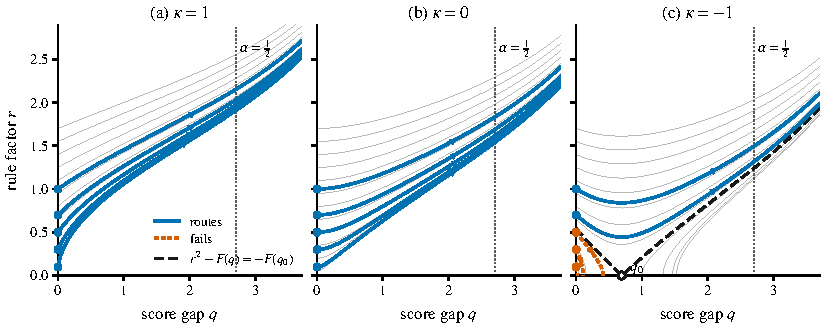
\includegraphics[width=\linewidth]{figures/phase_portrait.pdf}
\caption{Phase portrait of the reduced correlation-loss flow. $N=16$, $\eta=0.1$; grey curves are level sets of the invariant $r^2-F(q)$
(\cref{lem:invariant}), and trajectories start at $(0,\varepsilon)$ for $\varepsilon\in\{0.1,0.3,0.5,0.7,1\}$; the dotted line marks source attention $\alpha=1/2$.
(a)~Under $\Dlaw1$, $F$ is linear near $q=0$ and every trajectory leaves the axis at once; (b)~under $\Dlaw0$, $F(q)=q^2/2+O(q^3)$ and small-$\varepsilon$
trajectories creep along it. (c)~Under over-cancellation the rule first shrinks, and the separatrix $r^2-F(q)=-F(q_0)$ through $(q_0,0)$ divides routing from
collapse, the barrier $\varepsilon^2>-F(q_0)$ of \cref{thm:separation}(iii).}
\label{fig:phase}
\end{figure}


The proofs in \cref{app:routing-proof,app:critical} use one attention estimate, one primitive estimate, and the barrier minimum.

% ===================================================================
\section{Cross-entropy: escaping the bottleneck}
\label{sec:crossentropy}
Theorem~\ref{thm:separation}(iv) concerns the escape from uniform attention at fixed $N,\gamma$.
Cross-entropy preserves the matrix reduction and the score metric, but changes the rule gradient.
\emph{Proof idea.} With $m=r^2$, the exact derivatives give $m(q)=\Theta(\varepsilon^2+q^{2-\kappa})$ and $\ddt q=\Theta(m)$ on a small fixed
interval of $q$, for $\kappa\in\{0,1\}$, so the local hitting time is $\Theta(\int_0^b\frac{dq}{\varepsilon^2+q^{2-\kappa}})$: a logarithm for $\kappa=1$
and $1/\varepsilon$ for $\kappa=0$ (\cref{app:ce-proof}).

\paragraph{Beyond escape.}
For the anti-copy law the attended read takes many values, and at large rule product the cross-entropy score velocity
could in principle change sign before routing. We therefore do not claim complete cross-entropy routing as a theorem.
Numerically it completes in every tested configuration, with the score velocity bounded away from zero along each trajectory,
and the complete-routing times keep the two initialization orders (\cref{tab:network-flow,fig:network-flow}).

% ===================================================================
\section{Full-matrix training: a cross-entropy plateau}
\label{sec:fullmatrix}
\Cref{thm:separation} trains four tied scalars. Could a network whose every matrix entry trains escape the cancellation by learning other features,
other value maps or other attention patterns? Near the structured initialization it cannot. The proof needs no invariant manifold:
it combines the distributional cancellation of \cref{lem:matched} with a loss-floor and energy argument.

\paragraph{The full-matrix network.} Fix a residual width $d_{\mathrm{res}}\ge7$ and keep the embeddings and type mask of \cref{sec:architecture}, padded with
zeros to $\mathbb R^{d_{\mathrm{res}}}$. Every remaining entry is trainable: query and key $Q,K\in\mathbb R^{d\times d_{\mathrm{res}}}$, value $V\in\mathbb R^{d_v\times d_{\mathrm{res}}}$,
output $O\in\mathbb R^{d_{\mathrm{res}}\times d_v}$, MLP weights $U\in\mathbb R^{m\times d_{\mathrm{res}}}$, bias $\bm a\in\mathbb R^m$, $D\in\mathbb R^{d_{\mathrm{res}}\times m}$ and readout $\bm c\in\mathbb R^{d_{\mathrm{res}}}$,
with $d,d_v\ge1$ and $m\ge4$. The logit is
\begin{gather*}
 z_W=\bm c^\top\bigl[\bm g_b+D\relu(U\bm g_b+\bm a)\bigr],\qquad
 \bm g_b=\bm h_q^{(0)}+O\sum_{j=1}^N\alpha_jV\bm h_j^{(0)},\\
 \bm\alpha=\softmax\bigl((Q\bm h_q^{(0)})^\top K\bm h_j^{(0)}\bigr)_j .
\end{gather*}
Let $W_0$ be the matrices of \cref{eq:attention-matrices,eq:mlp-matrices} at $\bm\theta(0)$, padded with zeros, with readout $\bm c=\bm e_7$; nothing is tied afterwards.
Training follows $\dot W\in-\partial\mathcal L_{\mathrm{ce}}(W)$, the Clarke subgradient flow, which is ordinary gradient flow wherever the loss is differentiable.

\begin{mainresult}
\begin{theorem}[Full-matrix cross-entropy plateau]
\label{thm:fullmatrix}
Under $\Dlaw0$, let $B\ge1$, $C_B=110(B+2)$ and $0<\varepsilon\le1/10$. The constants do not depend on $d_{\mathrm{res}}$, $d$, $d_v$ or $m$.
\begin{enumerate}[label=(\roman*),leftmargin=*,itemsep=2pt,topsep=2pt]
\item \emph{Weak credit near initialization.} Every $W$ with $\|W-W_0\|_F\le\varepsilon$ has
$|\E[yz_W]|\le\gamma C_B\varepsilon^3$ and therefore $\mathcal L_{\mathrm{ce}}(W)\ge\log2-\gamma C_B\varepsilon^3/2$.
\item \emph{Plateau.} From $W(0)=W_0$, for all $0\le t<1/(C_B\varepsilon)$,
\[
 \|W(t)-W_0\|_F<\varepsilon,\qquad \mathcal L_{\mathrm{ce}}(W(t))\ge\log2-\tfrac12\gamma C_B\varepsilon^3 .
\]
Reaching any loss below $\log2-\delta$ with $\delta>\gamma C_B\varepsilon^3/2$ therefore takes time at least $1/(C_B\varepsilon)$.
\item \emph{Perturbed starts.} There is $L_B$ depending only on $B$ such that the same holds, with exit time at least $1/(4(C_B+(1+L_B)^2)\varepsilon)$,
from every $W(0)$ with $\|W(0)-W_0\|_F\le\varepsilon^{3/2}$.
\end{enumerate}
\end{theorem}
\end{mainresult}

\paragraph{Why the plateau holds.} At uniform attention the network sees only the instruction and the average embedding, which under $\Dlaw0$ is independent of the source, so
its logit has zero correlation with the label, whatever its other weights are (\cref{lem:matched}). Near $W_0$ attention can depart from uniform only by $O(\varepsilon)$,
and its dependence on the instruction, which the label needs, only by $O(\varepsilon^2)$: the key starts at zero and the query does not read the instruction.
Every path from attention to the logit passes through a product that starts at zero or at $O(\varepsilon)$, giving $|\E[yz_W]|=O(\varepsilon^3)$.
Cross-entropy equals $\log2-\E[yz]/2+\E\log\cosh(z/2)$, so the loss cannot fall by more than $O(\varepsilon^3)$ inside the ball, and the energy identity
$\|W(t)-W_0\|_F^2\le t\,[\mathcal L(W_0)-\mathcal L(W(t))]$ turns that into an exit time of order $1/\varepsilon$ (\cref{app:fullmatrix}).

\paragraph{Scope of the theorem.} It bounds the first exit under $\Dlaw0$ from an $\varepsilon$-ball around $W_0$, including starts perturbed by $\varepsilon^{3/2}$;
the exact rate and fast escape under $\Dlaw1$ are tested numerically in \cref{sec:numerics}, where the independent law leaves the ball in a time independent of $\varepsilon$.

% ===================================================================
\section{Causal corrupted reasoning traces}
\label{sec:causal}
The anti-copy laws also separate when $\eta=0$: there the mechanism is contextual correlation, rather than incorrect labels.
We now keep the instruction process fixed and make the error process itself create the correlations.
The same block is trained jointly on $N$ consecutive next-state predictions, each with local error rate $\eta>0$.

\paragraph{Construction.}
Fix $\eta\in(0,1/2)$, $\gamma=1-2\eta$, and $N\ge4$ such that
\[
 \frac{2}{N-1}<\min\{2\eta,\gamma\}.
\]
Start from $x_1=\cdots=x_N=w$, with $w$ uniform and $b_2=\cdots=b_N=1$.
For $i=N,\ldots,2N$, draw a fresh uniform $b_{i+1}$ and set $x_{i+1}=b_{i+1}x_i \xi_{i+1}$.
The two error regimes are
\begin{align}
 \text{independent:}\quad&\Pr(\xi_{i+1}=-1\mid\bm x_{<i+1},b_{i+1})=\eta,\notag\\
 \text{cancelling:}\quad&\Pr(\xi_{i+1}=-1\mid\bm x_{<i+1},b_{i+1})
 =\eta+\frac{b_{i+1}x_i\sum_{j=1}^i x_j}{2(N^2+N-i)}.
 \label{eq:causal-kernel}
\end{align}
Supervise every position $i=N+1,\ldots,2N$ with target $x_{i+1}$.
A fully correct control uses the same seed, instructions and supervised positions with $\xi_{i+1}=1$ at every step.

\begin{mainresult}\begin{theorem}[Wrong CoT steps generate credit cancellation]
\label{thm:causal}
For the construction above, compare the independent and cancelling error regimes.
Both regimes have uniform displayed-state marginals and, at every supervised position,
\[
 \Pr(x_{i+1}\ne b_{i+1}x_i\mid x_i,b_{i+1})=\eta,
 \qquad \hat x_{i+1}=b_{i+1}x_i
\]
as the Bayes predictor even given the full prefix.
Their cancellation coefficients are respectively
\[
 1+\sum_{j<i}\E[x_i x_j]=1\qquad\text{and}\qquad
 1+\sum_{j<i}\E[x_i x_j]=0.
\]
The complete trace has $2N$ transitions and expected incorrect fraction
$\eta(N+1)/(2N)\to\eta/2>0$.
More strongly, the number of incorrect transitions satisfies
\[
 N_{\mathrm w}\sim\operatorname{Binomial}(N+1,\eta),\qquad
 \Pr\!\left(\frac{N_{\mathrm w}}{2N}\ge\frac{\eta}{4}\right)
 \ge1-\exp\!\left(-\frac{\eta(N+1)}{8}\right).
\]
Train the same four coordinates from \cref{eq:initialization}, averaging correlation loss over these $N$ supervised prefixes.
Use the last visible state as source in each prefix and fix $B>\sqrt{\varepsilon^2+3\log(2N-1)}$ before training.
Let $T$ be the first time every supervised prefix has source attention at least $1/2$.
For $0<\varepsilon\le1$,
\begin{align*}
 T_{\mathrm{clean}}&=\Theta(N\log(1+\varepsilon^{-2})),&
 T_{\mathrm{independent}}&=\frac{T_{\mathrm{clean}}}{\gamma},\\
 T_{\mathrm{cancelling}}&=\Theta\!\left(\frac{N}{\gamma\varepsilon}\right),
\end{align*}
with absolute comparison constants. All three regimes reach the correct Bayes computation on a gate-valid interval beyond routing.
For fixed admissible $N,\eta$ and sufficiently small $\varepsilon$, $T_{\mathrm{cancelling}}>T_{\mathrm{independent}}>T_{\mathrm{clean}}$.
\end{theorem}\end{mainresult}
The cancelling kernel is a balancing bias. Its correction is proportional to $b_{i+1}x_i S_i$, the correct next state times the running sum of
displayed states, so a slip is slightly more likely when the correct step would extend the majority, and wrong steps keep the history balanced.
This is an existence result; whether natural reasoning errors cancel credit is an empirical question.
Exact balance is not required for the delay: within the anti-copy family, \cref{cor:dilution} keeps the order $1/\varepsilon$ for every
$\kappa\in[0,c\varepsilon]$.
\emph{Proof idea.} With $S_i=\sum_{j\le i}x_j$, averaging the fresh instruction in \cref{eq:causal-kernel} gives $\E[x_{i+1}\mid\bm x_{<i+1}]=-S_i/(N^2+N-i)$,
and induction from the seed gives $\E[x_{i+1}S_i]=-1$ and hence coefficient $0$ at every supervised position; independent errors make $x_{i+1}$ independent of its past (\cref{app:trace-proof}).
The condition on $N$ cannot hold at $\eta=0$, and the construction gives $\kappa=0$ for every admissible $\eta$, not an interpolation from the clean regime.
Its cancellation holds in conditional mean, weaker than the independence of \cref{lem:matched}; a causal process with distributional cancellation is left open.

% ===================================================================
\section{Experiments matched to the claims}
\label{sec:numerics}

All expectations are exact population sums; full results, tables and protocols are in \cref{app:experiments,app:repro}.

\paragraph{The theorem setting.} The matrix network reproduces the analytical gradients to $10^{-12}$, and gradient flow run through it by automatic differentiation
reproduces the reduced routing times to relative error $2\times10^{-9}$. Direct integration of the flow agrees with \cref{eq:time} to five significant figures, with invariant drift at most $6\times10^{-9}$;
reducing $\varepsilon$ tenfold multiplies $\Tr(\Dlaw0)$ by $10.3$ and $\Tr(\Dlaw1)$ by $1.5$, and over-cancellation follows the exact criterion of
\cref{thm:separation}(iii) (\cref{tab:quadrature}). Cross-entropy keeps both initialization orders for escape and complete routing
(\cref{tab:network-flow}), and with a clean fraction the routing time is within a factor $1.51$ of \cref{cor:dilution}.

\paragraph{Causal traces.} Exact propagation of the finite-state law checks every statement of \cref{thm:causal} for $\eta=0.2$ and $N\in\{8,16,32\}$.
At $N=16$, reducing $\varepsilon$ from $0.01$ to $0.001$ multiplies the routing time by $1.52$ with independent errors and by $10.26$ with cancelling errors (\cref{tab:causal-flow});
run through the causal network itself, the flow gives the same routing times to relative error $2\times10^{-11}$.

\paragraph{Untying and full matrices.} With every matrix entry trained from the theorem's directions with random magnitudes, the independent law learns
within $51$ time units, the anti-copy law slows roughly as $1/\varepsilon$ (from $24$ to $2{,}514$ time units as $\varepsilon$ falls from $0.3$ to $0.003$) or stalls under
added noise, and two anti-copies fail at every $\varepsilon\le0.3$ (\cref{tab:untied}). From exactly $W_0$, the full-matrix network leaves the $\varepsilon$-ball at flow time
$31.4/\varepsilon$ to $31.8/\varepsilon$ under the anti-copy law and at $23$ for every $\varepsilon$ under the independent law, as \cref{thm:fullmatrix} predicts; from starts perturbed by
$\varepsilon^{3/2}$ in every entry, at residual widths $7$, $16$ and $64$, the exits come at $20/\varepsilon$ to $27/\varepsilon$ and at $23$ respectively.

\paragraph{From fully random initialization.} With every matrix drawn at fan-in scale $\varepsilon$, the first escape from chance takes the same time under
every law, limited by the product of small weights. With Adam, all
$240$ independent-law runs reach the Bayes predictor, while $33$--$40\%$ of anti-copy runs and $43$--$50\%$ with two anti-copies stall at a flat stationary point
with clean accuracy $79$--$91\%$ (\cref{tab:randinit}). That point routes by instruction: for one sign of $b$ attention sits on the source and the prediction is Bayes
optimal, and for the other it puts no weight on the source and predicts as well as the decoys alone allow. This predicts the stalled accuracy and loss in every
law and context size to three decimals. Keeping the query, value and output matrices at order one gives the same picture, and a standard two-layer
Transformer separates the laws only under plain SGD (\cref{app:experiments}; under Adam, as \cref{rem:sign-flow} predicts, not at all), in the order of $|\kappa|$. This is what \cref{lem:credit} predicts once readout signs are free: at
uniform attention a path of either sign receives rule credit of size $|\kappa|$, and only under $\Dlaw0$ does every path receive none, for any readout (\cref{lem:matched}).
The fixed signs of \cref{eq:initialization} are what turn $\kappa<0$ into a barrier in \cref{thm:separation}.

% ===================================================================
\section{Discussion and limitations}
\label{sec:scope}
The model supplies the value direction, instruction interaction and source indicator. The matched laws share the local error rate and Bayes predictor, but their error probabilities given the complete prefix can differ.
The causal theorem trains all $N$ predictions after a supplied seed, its process is nonstationary, and its cancellation holds in conditional mean,
which is what the tied block reads, rather than in distribution.
The delay is proved near the structured initialization and observed when training starts from the specified directions; from fully random initialization
cancellation shows up as a higher rate of stalling at an instruction-split point (\cref{sec:numerics}), and we do not prove that the independent law escapes fast in full-matrix training.

% ===================================================================
\paragraph{Relation to prior work.}
\label{sec:related}

Corrupted chains of thought have been studied with static and propagated noise \citep{havrilla2024noise} and noisy rationales
\citep{zhou2024noisyrationales}; label-noise conditions \citep{natarajan2013noisy,patrini2017loss} address statistical recovery, and our matched laws differ in optimization.
Process supervision \citep{nye2021scratchpads,wei2022cot,uesato2022solving,lightman2023verify} has been analysed through statistical rates
\citep{jia2025verify,hanneke2026samplecomplexityautoregressivereasoning,pmlr-v291-joshi25a}, sparse dependence \citep{wen2024sparse} and parity \citep{kim2024parity}; we fix the format
and study its error structure. Weak-gradient and leap analyses \citep{shalevshwartz2017failures,abbe2025parities,abbe2021staircase,abbe2023sgd} tie slow learning
to weak target correlation; here that correlation is fixed and the sum over attended positions cancels, a data-induced analogue of deep-linear saddles
\citep{saxe2014exact,shamir2019exponential}. Attention plateaus also arise from rank growth \citep{boixadsera2023rank} and staged induction-head
formation \citep{bietti2023birth,reddy2024mechanistic,edelman2024evolution}, through architecture or a feature curriculum rather than data correlations.

% ===================================================================
\paragraph{Implications.}
\label{sec:conclusion}

Correct reasoning can survive incorrect chain-of-thought supervision, but learning time depends on how errors interact with attention:
independent errors weaken credit, while structured errors can cancel it and create an inverse-initialization bottleneck. Random initialization,
distributional cancellation in causal processes, and training without a supplied seed remain open.
            % abstract through conclusion

\bibliography{main}

\appendix
\crefalias{section}{appendix}

% !TEX root = main.tex
\section{Mathematical proofs}
\label{app:proofs}
The proofs start from \cref{eq:initialization} and use the Euclidean flow in \cref{eq:parameter-flow}.
Throughout, $N\ge4$, $\eta\in[0,\tfrac{1}{2})$, $\gamma=1-2\eta$, $\kappa\in[-1,1]$, and $0<\varepsilon\le1$.
The matrix reduction holds while $|r_1v|<2B$.
The fixed choice in \cref{eq:gate-bound} covers the correlation trajectory through $q=q_1+1$;
trapped trajectories have $r(t)\le \varepsilon$ for all time.
The cross-entropy proof establishes gate validity through complete routing. The causal theorem states its separate gate bound and prefix-size condition.

\subsection{Derivation from the one-block matrices}
\label{app:network-proof}
\label{app:architecture}
\paragraph{Embeddings and attention matrices.}
Let $\bm e_i\in\mathbb R^7$ be standard basis columns and let $\bm0$ denote a zero vector.
The state and query embeddings are
\begin{equation}
 \bm h_j^{(0)}=x_j\bm e_1+\bm e_3+\mathbf1[j=N]\bm e_4+\mathbf1[j<N]\bm e_5,
 \qquad \bm h_q^{(0)}=b\bm e_2+\bm e_3.
 \label{eq:embeddings}
\end{equation}
Here $\mathbf1[\cdot]$ is the indicator of the stated condition.
The one-dimensional query, key and value maps and their output projection are
\begin{equation}
 \begin{gathered}
 \bm w_q=\bm e_3^\top,\qquad
 \bm w_k=q_s\bm e_4^\top+q_d\bm e_5^\top,\qquad
 \bm w_v=\bm e_1^\top,\qquad \bm w_o=\bm e_6,\\
 \bm w_q,\bm w_k,\bm w_v\in\mathbb R^{1\times7},\qquad
 \bm w_o\in\mathbb R^{7\times1}.
 \end{gathered}
 \label{eq:attention-matrices}
\end{equation}
For the $N$ unmasked state positions, define the score vector $\bm q$ and attention vector $\bm\alpha$ by
\begin{equation}
 q_j=(\bm w_q\bm h_q^{(0)})(\bm w_k\bm h_j^{(0)}),\qquad
 \bm\alpha=\softmax(\bm q),\qquad
 \bm h_q=\bm h_q^{(0)}+\bm w_o\sum_{j=1}^N \alpha_j\bm w_v\bm h_j^{(0)}.
 \label{eq:attention-block}
\end{equation}
The query/key dimension is one, so the attention scaling factor is $1$.
The attended value is the scalar $v=\sum_j \alpha_j x_j$; the residual $\bm h_q$ is a vector.

\paragraph{Four-unit MLP matrices.}
Fix $B>0$, let $\bm1_4$ be the four-dimensional all-ones vector, and apply $\relu$ coordinatewise to vector arguments. Set
\begin{equation}
 \begin{gathered}
 \bm w_1=\begin{pmatrix}
 r_1\bm e_6^\top+B\bm e_2^\top\\
 -r_1\bm e_6^\top+B\bm e_2^\top\\
 r_1\bm e_6^\top-B\bm e_2^\top\\
 -r_1\bm e_6^\top-B\bm e_2^\top
 \end{pmatrix},\qquad
 \bm b_1=-B\bm1_4,\\
 \bm w_2=r_2\bm e_7(1,-1,-1,1),\qquad
 \bm w_1\in\mathbb R^{4\times7},\quad
 \bm w_2\in\mathbb R^{7\times4},\quad \bm b_1\in\mathbb R^4,\\
 \bm h'_q=\bm h_q+\bm w_2\relu(\bm w_1\bm h_q+\bm b_1),
 \qquad z=\bm e_7^\top\bm h'_q.
 \end{gathered}
 \label{eq:mlp-matrices}
\end{equation}

\begin{proof}[Proof of \cref{prop:realization}]
\proofstep{(a) Attention.}
For the embeddings and matrices above,
\begin{align*}
 \bm w_q\bm h_q^{(0)}&=1,&
 \bm w_k\bm h_j^{(0)}&=q_s\mathbf1[j=N]+q_d\mathbf1[j<N],&
 \bm w_v\bm h_j^{(0)}&=x_j,\\
 \bm h_q&=\bm h_q^{(0)}+\bm e_6\sum_{j=1}^N \alpha_j x_j,&
 \alpha(q)&=\frac{e^{q_s}}{e^{q_s}+(N-1)e^{q_d}}
 =\frac{e^q}{e^q+N-1}.
\end{align*}
Every decoy has weight $\tfrac{1-\alpha(q)}{N-1}$, so with $\bar w=\tfrac{1}{N-1}\sum_{j<N}x_j$,
\[
 v=\sum_{j=1}^N \alpha_j x_j=\alpha(q)x_N+(1-\alpha(q))\bar w,\qquad |v|\le1.
\]
\proofstep{(b) MLP.}
The preactivation is
\[
 \bm w_1\bm h_q+\bm b_1=
 \begin{pmatrix}
 r_1v+B(b-1)\\-r_1v+B(b-1)\\
 r_1v-B(b+1)\\-r_1v-B(b+1)
 \end{pmatrix}.
\]
Since $\bm e_7^\top\bm h_q=0$ and $|r_1v|<2B$,
\begin{align*}
 b=1:\quad z&=r_2\bigl[\relu(r_1v)-\relu(-r_1v)\bigr]=r_1r_2v,\\
 b=-1:\quad z&=r_2\bigl[-\relu(r_1v)+\relu(-r_1v)\bigr]=-r_1r_2v.
\end{align*}
Thus $z=r_1r_2b v$ on the open gate-valid region.
\proofstep{(c) Parameter gradients.}
For each coordinate $\theta_i$ of $\bm\theta$, differentiation of the identity gives
\begin{align*}
 \pd{}{\theta_i}\E[\ell(y,z)]
 &=\E\left[\pd{\ell}{z}(y,z)\pd{z}{\theta_i}\right]&&\text{(finite support; chain rule)}\\
 &=\E\left[\pd{\ell}{z}(y,r_1r_2b v)\pd{(r_1r_2b v)}{\theta_i}\right]
 =\pd{}{\theta_i}\E[\ell(y,r_1r_2b v)].
\end{align*}
Stacking the four coordinates yields equality of $\nabla_{\bm\theta}$ for the matrix network and its derived logit.
The matrix chain rule, for example, is
\[
 \pd{\mathcal L}{r_1}=\left\langle\nabla_{\bm w_1}\mathcal L,\pd{\bm w_1}{r_1}\right\rangle_{\mathrm F},\qquad
 \pd{\mathcal L}{r_2}=\left\langle\nabla_{\bm w_2}\mathcal L,\pd{\bm w_2}{r_2}\right\rangle_{\mathrm F}.
\]
At $r_1v=0$, the composite $\relu(z)-\relu(-z)=z$ remains differentiable.
Assigning derivative $\tfrac{1}{2}$ to each paired ReLU at zero reproduces its derivative $1$.\qedhere
\end{proof}

\subsection{Cancellation and matched laws}
\label{app:credit-proof}
\begin{proof}[Proof of \cref{lem:credit}]
\proofstep{(a) Factorization.}
Substitute $y=b x_N\xi$:
\begin{align*}
 \E[y b x_j]&=\E[\xi]\E[x_N x_j]=\gamma\E[x_N x_j]
 &&\text{(independence; $b^2=1$)},\\
 \E[y b x_N]&=\gamma
 &&\text{($x_N^2=1$)}.
\end{align*}
\proofstep{(b) Uniform initialization.}
At $\bm q=\bm0$, $\alpha_j=\tfrac{1}{N}$ and
\begin{align*}
 -\pd{\mathcal L}{r_1}
 &=\frac{r_2}{2}\E[y b v]
 =\frac{r_2}{2N}\left(\E[y b x_N]+\sum_{j=1}^{N-1}\E[y b x_j]\right)\\
 &=\frac{r_2\gamma}{2N}\left(1+\sum_{j=1}^{N-1}\E[x_N x_j]\right)
 =\frac{r_2\gamma \kappa}{2N}&&\text{(definition of $\kappa$)}.
\end{align*}
Exchange $r_1,r_2$ for the other rule factor.
Under $\Dlaw{\kappa}$, a decoy is an anti-copy with probability $\tfrac{\E[M]}{N-1}=\rho$ and is otherwise independent of $x_N$, so
$\E[x_N x_j]=-\rho$ and $1+\sum_{j=1}^{N-1}\E[x_N x_j]=1-(N-1)\rho=\kappa$.\qedhere
\end{proof}

\begin{proof}[Proof of \cref{lem:matched}]
\proofstep{(a) Marginals and conditional prediction.}
The law is invariant under the global sign flip $(x_1,\ldots,x_N)\mapsto(-x_1,\ldots,-x_N)$, so every displayed sign is uniform.
Independence of $b,\xi$ from the prefix gives
\begin{align*}
 \Pr(y=b x_N\mid\bm x_{<N+1},b)&=1-\eta,\\
 \Pr(y=-b x_N\mid\bm x_{<N+1},b)&=\eta<\frac{1}{2},\\
 \operatorname*{argmax}_{y\in\{-1,1\}}\Pr(y\mid\bm x_{<N+1},b)&=b x_N.
\end{align*}
\proofstep{(b) One anti-copy.}
The conditional law of $(b,y)$ given the prefix is common to all the laws, so total variation is that of the prefixes;
$x_N$ is uniform under each law, so it is the average over $x_N$ of the total variation of the decoy vectors given $x_N$.
Write $\Dlaw{(m)}$ for the law with exactly $m$ anti-copies and fix $x_N$.
Under $\Dlaw{(0)}=\Dlaw1$ every decoy vector $\bm d\in\{-1,1\}^{N-1}$ has mass $2^{-(N-1)}$.
Under $\Dlaw{(1)}=\Dlaw0$, $\bm d$ arises once for each of its $K(\bm d)$ coordinates equal to $-x_N$, so its mass is
$\tfrac{K(\bm d)}{N-1}2^{-(N-2)}$. With $K$ distributed as under $\Dlaw1$ and $2K-(N-1)=-x_N\sum_{j<N}x_j$,
\[
 d_{\mathrm{TV}}(\Dlaw0,\Dlaw1)=\frac{1}{2}\E_{\Dlaw1}\left|\frac{2K}{N-1}-1\right|
 =\frac{\E|S_{N-1}|}{2(N-1)}=\tau_N\le\frac{\sqrt{N-1}}{2(N-1)},
\]
using $\E|S_{N-1}|\le(\E S_{N-1}^2)^{1/2}$.
The same computation with $N-2$ free decoys compares one further anti-copy with an independent decoy:
$d_{\mathrm{TV}}(\Dlaw{(2)},\Dlaw{(1)})\le\tfrac{1}{2\sqrt{N-2}}$.
\proofstep{(c) Mixtures.}
For $0\le\kappa\le1$, $\Dlaw{\kappa}=\kappa\Dlaw1+(1-\kappa)\Dlaw0$, so
$d_{\mathrm{TV}}(\Dlaw{\kappa},\Dlaw1)=(1-\kappa)\,d_{\mathrm{TV}}(\Dlaw0,\Dlaw1)=(1-\kappa)\tau_N$.
For $-1\le\kappa<0$, $\Dlaw{\kappa}=(1+\kappa)\Dlaw0+(-\kappa)\Dlaw{(2)}$, and the triangle inequality gives
\[
 d_{\mathrm{TV}}(\Dlaw{\kappa},\Dlaw1)\le d_{\mathrm{TV}}(\Dlaw0,\Dlaw1)+(-\kappa)\,d_{\mathrm{TV}}(\Dlaw{(2)},\Dlaw0)
 \le\frac{1-\kappa}{2\sqrt{N-2}}.
\]
\proofstep{(d) Distributional cancellation.}
Under $\Dlaw0$ the multiset of displayed values consists of $x_N$, its anti-copy $-x_N$, and $N-2$ independent uniform signs,
that is, of one $+1$, one $-1$ and $N-2$ independent uniform signs, whatever $x_N$ is.
Hence the multiset is independent of $x_N$; since $b$ and $\xi$ are independent of the prefix, $x_N$ is uniform given $(b,\{x_1,\ldots,x_N\})$,
and so is $y=b x_N\xi$. Under $\Dlaw1$, $\E[y b x_N]=\E[\xi]=\gamma$.\qedhere
\end{proof}

\subsection{From initialization to routing and prediction}
\label{app:flow-proof}
\begin{proof}[Proof of \cref{lem:invariant}]
\proofstep{(a) Balanced trajectory.}
Under $\Dlaw{\kappa}$, $\E[x_N\bar w]=-\rho$ (\cref{lem:credit}), so
$\E[y b v]=\gamma[\alpha(q)-(1-\alpha(q))\rho]=\gamma \phi(q)$. Therefore
\begin{align}
 \mathcal L&=-\frac{\gamma}{2}r_1r_2\phi(q),\notag\\
 \ddt{r_1}&=\frac{\gamma}{2}r_2\phi,&\ddt{r_2}&=\frac{\gamma}{2}r_1\phi,\label{eq:four-scalar-flow}\\
 \ddt{q_s}&=\frac{\gamma}{2}r_1r_2\phi'(q),&
 \ddt{q_d}&=-\frac{\gamma}{2}r_1r_2\phi'(q).\notag
\end{align}
The initialization in \cref{eq:initialization} and uniqueness imply
\begin{align*}
 \frac{d}{dt}(r_1-r_2)&=-\frac{\gamma}{2}\phi(q)(r_1-r_2),&(r_1-r_2)(0)&=0,\\
 \frac{d}{dt}(q_s+q_d)&=0,&(q_s+q_d)(0)&=0.
\end{align*}
Consequently $r_1=r_2=r$, $q_s=-q_d=\tfrac{q}{2}$, and
\begin{equation}
 r(t)=\varepsilon\exp\left(\frac{\gamma}{2}\int_0^t \phi(q(v))\,dv\right)>0,\qquad
 \ddt{q}=\gamma r^2\phi'(q)>0.
 \label{eq:balanced-flow}
\end{equation}
For finite $t$, $|\phi|\le1$, $\phi'(q)\le\tfrac{1+\rho}{4}$ give
\[
 \varepsilon e^{-\frac{\gamma t}{2}}\le r(t)\le \varepsilon e^{\frac{\gamma t}{2}},\qquad
 q(t)\le\frac{\gamma(1+\rho)\varepsilon^2}{4}\int_0^t e^{\gamma v}\,dv<\infty.
\]
These bounds exclude finite-time escape of the derived smooth vector field.
\proofstep{(b) Conserved quantity.}
Set $\alpha_0=\tfrac{\rho}{1+\rho}$ for this calculation only. Then
\begin{align}
 \dv{\alpha(q)}{q}&=\alpha(q)(1-\alpha(q)),&
 \frac{\phi(q)}{\phi'(q)}&=\frac{\alpha(q)-\alpha_0}{\alpha(q)(1-\alpha(q))},\notag\\
 F(q)&=\int_{\tfrac{1}{N}}^{\alpha(q)}\frac{\alpha-\alpha_0}{\alpha^2(1-\alpha)^2}\,d\alpha.\label{eq:primitive}
\end{align}
\begin{align*}
 \frac{d}{dt}(r^2-F(q))
 &=\gamma r^2\phi-\frac{\phi}{\phi'(q)}\gamma r^2\phi'(q)
 &&\text{(chain rule)},\\
 &=0 &&\text{(cancellation)}.
\end{align*}
At initialization $F(0)=0$; hence $r(t)^2=\varepsilon^2+F(q(t))$.
\proofstep{(c) Hitting time.}
If $\varepsilon^2+F>0$ on $[0,b]$, compactness gives
\[
 \min_{0\le q\le b}\gamma(\varepsilon^2+F(q))\phi'(q)>0.
\]
Thus the increasing score gap reaches $b$ in finite time and
\begin{equation}
 T(b)=\int_0^b\frac{dq}{\gamma(\varepsilon^2+F(q))\phi'(q)}.
 \label{eq:hitting-quadrature}
\end{equation}
Taking $b=q_1$ proves \cref{eq:time}.
\proofstep{(d) Gate validity and prediction.}
Since $\alpha_0\ge0$,
\begin{align*}
 \dv{F(q)}{q}&\le\frac{1}{1-\alpha(q)}=1+\frac{e^q}{N-1},\\
 F(q)&\le q+\frac{e^q-1}{N-1}
 <\log(N-1)+1+e\qquad(0\le q\le q_1+1).
\end{align*}
Therefore \cref{eq:gate-bound} gives $|r_1v|\le r<2B$ throughout this interval.
For $\kappa\in\{0,1\}$, $\phi(q)\ge0$ and $F(q)\ge0$ for $q\ge0$; part (c) gives $T(q_1+1)<\infty$.
At $q>q_1$,
\[
 x_N v=\alpha(q)+(1-\alpha(q))x_N\bar w\ge2\alpha(q)-1>0,
 \qquad \operatorname{sign}(z)=b x_N.
\]
Thus the network reaches the Bayes predictor in finite time and retains it through the stopping gap $q_1+1$.\qedhere
\end{proof}

\subsection{Routing-time estimates}
\label{app:routing-proof}
Write $q_1=\log(N-1)$; $N\ge4$ implies $q_1>1$.
The quantitative bounds in parts (i)--(ii) of \cref{thm:separation} are
\begin{align*}
 \frac{N-1}{2e\gamma}\log\!\left(1+\frac{2}{\varepsilon^2}\right)
 &\le\Tr(\Dlaw1)\le\frac{4(N-1)}{\gamma}\left[\log(1+\varepsilon^{-2})+\frac{1}{e}\right],\\
 \frac{N-1}{5\gamma \varepsilon}
 &\le\Tr(\Dlaw0)\le\frac{4(N-1)}{\gamma}\left[\frac{\sqrt2\pi}{\varepsilon}+\frac{8}{e}\right].
\end{align*}

\begin{lemma}[Attention bounds on the routing interval]
\label{lem:attention-bounds}
For $q\in[0,q_1]$,
\begin{equation}
 \frac{e^q}{2(N-1)}\le \alpha(q)\le\frac{e^q}{N},\qquad
 \frac{1}{N}\le \alpha(q)\le\frac{1}{2},\qquad
 \phi'(q)\ge\frac{e^q}{4(N-1)}.
 \label{eq:alpha-bounds}
\end{equation}
For $\kappa\in\{0,1\}$ and $q\in[0,1]$, $\phi'(q)\le \tfrac{e}{N-1}$.
\end{lemma}
\begin{proof}
\begin{align*}
 1\le e^q\le N-1
 &\quad\Longrightarrow\quad
 N\le e^q+N-1\le2(N-1),\\
 \phi'(q)=(1+\rho)\alpha(q)(1-\alpha(q))
 &\ge\frac{\alpha(q)}{2}\ge\frac{e^q}{4(N-1)}&&\text{($\rho\ge0$, $\alpha\le\tfrac12$)},\\
 \kappa\in\{0,1\},\ 0\le q\le1:\quad
 \phi'(q)&\le(1+\rho)\alpha(q)
 \le\frac{N}{N-1}\frac{e^q}{N}\le\frac{e}{N-1}.\qedhere
\end{align*}
\end{proof}

\begin{lemma}[Primitive bounds]
\label{lem:primitive-bounds}
For $0\le q\le q_1$, the two laws satisfy
\begin{align}
 \kappa=1:\quad &q\le F(q)\le2q,\label{eq:ordinary-primitive-bounds}\\
 \kappa=0:\quad &\frac{q^2}{8}\le F(q)\le2q^2\quad(0\le q\le1),\qquad
 F(q)\ge\frac{1}{8}\quad(1\le q\le q_1).
 \label{eq:cancelled-primitive-bounds}
\end{align}
\end{lemma}
\begin{proof}
\proofstep{(a) Ordinary law.}

Here $\rho=0$, $\phi=\alpha$, and $\phi'(q)=\alpha(1-\alpha)$.
\Cref{lem:attention-bounds} gives $1\le \tfrac{\phi}{\phi'(q)}\le2$;
$F(q)=\int_0^q\tfrac{\phi(v)}{\phi'(v)}\,dv\in[q,2q]$.

\proofstep{(b) Cancelled law.}

Here $\rho=\tfrac{1}{N-1}$, and
\[
 \dv{F(q)}{q}=\frac{\alpha(q)-\frac{1}{N}}{\alpha(q)(1-\alpha(q))}\ge0\quad(q\ge0).
\]
For $0\le q\le1$, \cref{lem:attention-bounds} and convexity give
\begin{align*}
 \alpha(q)-\frac{1}{N}
 &=\frac{(e^q-1)(N-1)}{N(e^q+N-1)}\le\frac{e^q-1}{N},\\
 \alpha(q)(1-\alpha(q))&\ge\frac{1}{2N},&
 e^q-1&\le(e-1)q\le2q,\\
 \dv{F(q)}{q}&\le4q,&F(q)&\le2q^2.
\end{align*}
For $0\le q\le q_1$,
\begin{align*}
 \dv{F(q)}{q}&\ge\frac{\alpha(q)-\frac{1}{N}}{\alpha(q)}
 =\frac{N-1}{N}(1-e^{-q})\ge\frac{1}{2}(1-e^{-q}),\\
 0\le q\le1:\quad
 1-e^{-q}&\ge q-\frac{q^2}{2}\ge \frac{q}{2},\\
 F(q)&\ge\int_0^q \frac{v}{4}\,dv=\frac{q^2}{8},\\
 q\ge1:\quad F(q)&\ge F(1)\ge\frac{1}{8}&&\text{($F$ is nondecreasing)}.\qedhere
\end{align*}
\end{proof}

\begin{proof}[Proof of \cref{thm:separation}(i) and \cref{rem:rescaling}]
For a fixed displayed-prefix law and independent error sign, write $\mathcal L_\eta$ for correlation loss. Then
\[
 \mathcal L_\eta(\bm\theta)=(1-2\eta)\mathcal L_0(\bm\theta),\qquad
 \bm\theta_\eta(t)=\bm\theta_0((1-2\eta)t),\qquad
 T(\eta,\kappa)=\frac{T(0,\kappa)}{1-2\eta}.
\]
The trajectory identity follows from the chain rule and uniqueness in the original Euclidean coordinate metric.
It holds on corresponding gate-valid intervals, with infinite routing times interpreted as infinite.
Thus independent corruption at fixed $\kappa=1$ strictly increases finite routing time for $\eta>0$;
the failure threshold at fixed $\kappa<0$ is unchanged.

By \cref{lem:primitive-bounds}, $\varepsilon^2+F(q)>0$ on $[0,q_1]$.
\Cref{lem:invariant,lem:attention-bounds,lem:primitive-bounds} give
\begin{align*}
 \Tr
 &\le\frac{4(N-1)}{\gamma}\int_0^{q_1}\frac{e^{-q}}{\varepsilon^2+q}\,dq\\
 &\le\frac{4(N-1)}{\gamma}
 \left(\int_0^1\frac{dq}{\varepsilon^2+q}+\int_1^\infty e^{-q}\,dq\right)\\
 &=\frac{4(N-1)}{\gamma}\left(\log(1+\varepsilon^{-2})+e^{-1}\right),\\[2pt]
 \Tr
 &\ge\frac{N-1}{e\gamma}\int_0^1\frac{dq}{\varepsilon^2+2q}
 =\frac{N-1}{2e\gamma}\log(1+2\varepsilon^{-2}).\qedhere
\end{align*}
\end{proof}

\begin{proof}[Proof of \cref{thm:separation}(ii)]
By \cref{lem:primitive-bounds}, $\varepsilon^2+F(q)\ge \varepsilon^2>0$.
\Cref{lem:invariant,lem:attention-bounds,lem:primitive-bounds} give
\begin{align*}
 \Tr
 &\ge\frac{N-1}{e\gamma}\int_0^1\frac{dq}{\varepsilon^2+2q^2}
 =\frac{N-1}{e\gamma}\frac{\arctan(\frac{\sqrt2}{\varepsilon})}{\sqrt2\varepsilon}
 \ge\frac{N-1}{\gamma \varepsilon}\frac{\arctan\sqrt2}{\sqrt2e},\\
 \arctan\sqrt2
 &=\int_0^1\frac{dv}{1+v^2}+\int_1^{\sqrt2}\frac{dv}{1+v^2}\\
 &\ge\int_0^1(1-v^2)\,dv+\frac{\sqrt2-1}{3}=\frac{1+\sqrt2}{3},\\
 \sqrt2<\frac{3}{2},\ e<\frac{11}{4}
 &\quad\Longrightarrow\quad
 \frac{\arctan\sqrt2}{\sqrt2e}>\frac{20}{99}>\frac{1}{5},\\[2pt]
 \Tr
 &\le\frac{4(N-1)}{\gamma}
 \left(\int_0^1\frac{dq}{\varepsilon^2+\frac{q^2}{8}}+8\int_1^{q_1}e^{-q}\,dq\right)\\
 &\le\frac{4(N-1)}{\gamma}
 \left(\int_0^\infty\frac{dq}{\varepsilon^2+\frac{q^2}{8}}+8e^{-1}\right)\\
 &=\frac{4(N-1)}{\gamma}
 \left(\frac{\sqrt2\pi}{\varepsilon}+\frac{8}{e}\right).\qedhere
\end{align*}
\end{proof}

\subsection{Diluted cancellation: proof of \texorpdfstring{\cref{cor:dilution}}{the dilution corollary}}
\label{app:dilution}
\begin{proof}[Proof of \cref{cor:dilution}]
For $0\le\lambda\le1$, \cref{def:Dkappa} draws $M\sim\mathrm{Bernoulli}(1-\lambda)$ anti-copies, so $\Dlaw\lambda=\lambda\Dlaw1+(1-\lambda)\Dlaw0$.
Write $\kappa=\lambda$, $\rho=\tfrac{1-\lambda}{N-1}$ and $\alpha_0=\tfrac{\rho}{1+\rho}=\tfrac{1-\lambda}{N-\lambda}$.
\proofstep{(a) The primitive.}
From \cref{eq:primitive}, $F'(q)=\tfrac{\alpha(q)-\alpha_0}{\alpha(q)(1-\alpha(q))}=\tfrac{g(q)}{1-\alpha(q)}$ with
\[
 g(q)=1-\frac{\alpha_0}{\alpha(q)}=\frac{N-1}{N-\lambda}\Bigl[\lambda+(1-\lambda)(1-e^{-q})\Bigr]\ge0 .
\]
On $[0,q_1]$, $1\le\tfrac{1}{1-\alpha(q)}\le2$, and $\tfrac{N-1}{N-\lambda}\in[\tfrac{3}{4},1]$. For $0\le q\le1$, $\tfrac{q}{2}\le1-e^{-q}\le q$, and
$\lambda+(1-\lambda)q\ge\tfrac{\lambda+q}{4}$ (if $\lambda\le\tfrac12$ the left side is at least $\lambda+\tfrac{q}{2}$; otherwise it is at least $\lambda>\tfrac12\ge\tfrac{\lambda+q}{4}$). Hence
\[
 \frac{3}{32}(\lambda+q)\le F'(q)\le2(\lambda+q),\qquad
 \frac{3}{32}\Bigl(\lambda q+\frac{q^2}{2}\Bigr)\le F(q)\le2\Bigl(\lambda q+\frac{q^2}{2}\Bigr)\qquad(0\le q\le1),
\]
and, since $F$ is nondecreasing, $F(q)\ge F(1)\ge\tfrac{3}{64}$ on $[1,q_1]$.
\proofstep{(b) Time bounds.}
\Cref{lem:attention-bounds} gives $\phi'(q)\ge\tfrac{e^q}{4(N-1)}$ on $[0,q_1]$, and its upper bound $\phi'(q)\le(1+\rho)\alpha(q)\le\tfrac{e}{N-1}$ on $[0,1]$ holds for every $\lambda\in[0,1]$ because $1+\rho\le\tfrac{N}{N-1}$.
Write $I=\int_0^1\tfrac{dq}{\varepsilon^2+\lambda q+q^2}$; note $I\ge\tfrac{1}{3}$. Using $\varepsilon^2+F\le2(\varepsilon^2+\lambda q+q^2)$ and $\varepsilon^2+F\ge\tfrac{3}{64}(\varepsilon^2+\lambda q+q^2)$ on $[0,1]$, \cref{eq:time} gives
\begin{align*}
 \Tr&\ge\frac{N-1}{e\gamma}\int_0^1\frac{dq}{\varepsilon^2+F(q)}\ge\frac{N-1}{2e\gamma}\,I,\\
 \Tr&\le\frac{4(N-1)}{\gamma}\left(\int_0^1\frac{e^{-q}\,dq}{\varepsilon^2+F(q)}+\int_1^{q_1}\frac{e^{-q}\,dq}{F(1)}\right)\\
 &\le\frac{256(N-1)}{3\gamma}\bigl(I+e^{-1}\bigr)\le\frac{256(1+3e^{-1})(N-1)}{3\gamma}\,I .
\end{align*}
\proofstep{(c) The integral.}
Since $\max\{a,b,c\}\le a+b+c\le3\max\{a,b,c\}$, $I$ is within a factor $3$ of $J=\int_0^1\tfrac{dq}{\max\{\varepsilon^2,\lambda q,q^2\}}$.
If $\lambda\le\varepsilon$, then $\lambda q\le\max\{\varepsilon^2,q^2\}$ and $J=\tfrac{2}{\varepsilon}-1\in[\tfrac{1}{\varepsilon},\tfrac{2}{\varepsilon}]$.
If $\lambda>\varepsilon$, the three regimes meet at $q=\tfrac{\varepsilon^2}{\lambda}<\lambda\le1$, and
\[
 J=\frac{1}{\lambda}+\frac{2}{\lambda}\log\frac{\lambda}{\varepsilon}+\frac{1}{\lambda}-1
 \in\left[\frac{1+2\log(\lambda/\varepsilon)}{\lambda},\ \frac{2+2\log(\lambda/\varepsilon)}{\lambda}\right].
\]
With $C=\tfrac{1+\log(1+\lambda/\varepsilon)}{\lambda}$: for $\lambda\le\varepsilon$, $C\ge\tfrac{1}{\lambda}\ge\tfrac{1}{\varepsilon}$, so $\min\{\tfrac{1}{\varepsilon},C\}=\tfrac{1}{\varepsilon}$;
for $\lambda>\varepsilon$, $\log\tfrac{\lambda}{\varepsilon}\le\log(1+\tfrac{\lambda}{\varepsilon})\le\log\tfrac{\lambda}{\varepsilon}+\log2$ and $C\le\tfrac{1+\log2}{\varepsilon}$.
In both cases $J$, and hence $I$, is within absolute constants of $\min\{\tfrac{1}{\varepsilon},C\}$; with part (b) this proves the corollary.
\end{proof}
Numerically, $F(q)/(\lambda q+\tfrac{q^2}{2})\in[0.67,1.14]$ on $[0,1]$ for $N\in\{8,16,64,256\}$, and
$\tfrac{\gamma\Tr}{(N-1)I}\in[1.03,1.51]$ over $N\in\{16,64\}$, $\varepsilon\in\{10^{-2},10^{-3},10^{-4}\}$ and eleven values of $\lambda\in[0,1]$, well inside the proved constants.

\subsection{Over-cancellation: exact barrier and critical equality}
\label{app:critical}

\begin{lemma}[Barrier location and size]
\label{lem:barrier}
For $-1\le \kappa<0$, let $\alpha_0=\tfrac{1+|\kappa|}{N+|\kappa|}$ and $q_0=\log(1-\kappa)$.
Then $\phi(q_0)=0$, $\alpha(q_0)=\alpha_0$, and
\begin{equation}
 \min_{q\ge0}F(q)=F(q_0)<0,\qquad
 \frac{9\kappa^2}{200}\le -F(q_0)\le2\kappa^2,\qquad
 \frac{1}{N}<\alpha_0\le\frac{2}{N}.
 \label{eq:barrier-bounds}
\end{equation}
\end{lemma}
\begin{proof}
\proofstep{(a) Location and sign.}
\begin{align*}
 \frac{(N-1)\alpha_0}{1-\alpha_0}&=(N-1)\rho=1-\kappa,\\
 \dv{F(q)}{q}&=\frac{\alpha(q)-\alpha_0}{\alpha(q)(1-\alpha(q))},\\
 q<q_0&\Rightarrow \dv{F(q)}{q}<0,&q>q_0&\Rightarrow \dv{F(q)}{q}>0,\\
 |\kappa|(N-2)\le N&\Rightarrow \alpha_0\le\frac{2}{N}.
\end{align*}
\proofstep{(b) Lower bound.}
\begin{align*}
 -F(q_0)
 &=\int_{\frac{1}{N}}^{\alpha_0}\frac{\alpha_0-\alpha}{\alpha^2(1-\alpha)^2}\,d\alpha
 \ge\frac{(\alpha_0-\frac{1}{N})^2}{2\alpha_0^2}
 =\frac{(N \alpha_0-1)^2}{2(N \alpha_0)^2},\\
 N \alpha_0-1&=\frac{|\kappa|(N-1)}{N+|\kappa|}\ge\frac{3}{5}|\kappa|,&N \alpha_0&\le2,\\
 -F(q_0)&\ge\frac{9\kappa^2}{200}.
\end{align*}
\proofstep{(c) Upper bound.}
For $\alpha\in[\tfrac{1}{N},\alpha_0]$,
\begin{align*}
 \alpha^2(1-\alpha)^2&\ge\frac{(1-\alpha_0)^2}{N^2}\ge\frac{1}{4N^2},\\
 -F(q_0)&\le4N^2\int_{\frac{1}{N}}^{\alpha_0}(\alpha_0-\alpha)\,d\alpha
 =2(N \alpha_0-1)^2\le2\kappa^2.\qedhere
\end{align*}
\end{proof}

The failure part also yields the following quantitative conclusions.
Below this barrier, $q(t)\uparrow q_z<q_0$ and $r(t)\to0$, where $q_z$ is the unique root of $\varepsilon^2+F(q_z)=0$.
At equality, $q(t)\uparrow q_0$ and $r(t)\downarrow0$.
Both failure cases have $\alpha(q(t))<\tfrac{2}{N}$ for every finite $t$.
Moreover $\tfrac{9\kappa^2}{200}\le-F(q_0)\le2\kappa^2$;
$\varepsilon\le\tfrac{|\kappa|}{9}$ suffices for failure, and $\varepsilon>\sqrt2|\kappa|$ suffices for routing.
\begin{proof}[Proof of \cref{thm:separation}(iii)]
\proofstep{(a) Above the barrier.}
If $\varepsilon^2>-F(q_0)$, then $\min_{[0,q_1]}(\varepsilon^2+F)>0$ by \cref{lem:barrier}; \cref{lem:invariant} gives $\Tr<\infty$.
\proofstep{(b) Below the barrier.}

\Cref{lem:barrier} gives strict decrease of $F$ on $[0,q_0]$, with
$\varepsilon^2+F(0)>0>\varepsilon^2+F(q_0)$; hence $q_z$ exists uniquely.
By \cref{lem:invariant},
\[
 r(t)>0,\qquad r(t)^2=\varepsilon^2+F(q(t)),\qquad\ddt{q}>0
 \quad\Longrightarrow\quad 0\le q(t)<q_z.
\]
Let $q_\infty=\lim_{t\to\infty}q(t)\le q_z$.
If $q_\infty<q_z$, then
\[
 \ddt{q}(t)\ge\min_{0\le q\le q_\infty}
 \gamma(\varepsilon^2+F(q))\phi'(q)>0,
\]
so $q(t)\to\infty$, a contradiction. Therefore $q_\infty=q_z$ and
$r(t)^2\to \varepsilon^2+F(q_z)=0$.

\proofstep{(c) Equality.}

At $q=q_0$, $\phi=0$ and
\begin{align*}
 \left.\dv{F(q)}{q}\right|_{q=q_0}&=0,\\
 \left.\frac{d^2F(q)}{dq^2}\right|_{q=q_0}
 &=\left.\dv{}{q}\left(\frac{\phi(q)}{\phi'(q)}\right)\right|_{q=q_0}\\
 &=\left.\left[1-\frac{\phi(q)\phi''(q)}{\bigl(\phi'(q)\bigr)^2}\right]\right|_{q=q_0}=1.
\end{align*}
Taylor's theorem gives $b>0$ such that, for $q_0-b\le q\le q_0$,
\[
 \frac{1}{4}(q-q_0)^2\le F(q)-F(q_0)\le\frac{3}{4}(q-q_0)^2.
\]
On $[0,q_0]$, $\phi'(q)\le\tfrac{1+\rho}{4}$, so
\[
 \int_{q_0-b}^{q_0}\frac{dq}{\gamma[\varepsilon^2+F(q)]\phi'(q)}
 \ge\frac{16}{3\gamma(1+\rho)}\int_{q_0-b}^{q_0}\frac{dq}{(q-q_0)^2}=\infty.
\]
Thus $q(t)<q_0$ at every finite time.
The same bounded-monotone limit argument as in part (b) yields
$q(t)\uparrow q_0$ and $r(t)^2\to \varepsilon^2+F(q_0)=0$.
Since $\phi(q)<0$ for $q<q_0$, $\ddt{r}<0$.
\proofstep{(d) Attention and sufficient conditions.}
Finally $q_0=\log(1-\kappa)\le\log2<\log(N-1)=q_1$, so routing fails. In both failure cases $\alpha(q(t))<\alpha(q_0)=\alpha_0\le\tfrac{2}{N}$.
The bounds in \cref{lem:barrier} give
\[
 \varepsilon\le\frac{|\kappa|}{9}\ \Longrightarrow\ \varepsilon^2<\frac{9\kappa^2}{200}\le-F(q_0),\qquad
 \varepsilon>\sqrt2|\kappa|\ \Longrightarrow\ \varepsilon^2>2\kappa^2\ge-F(q_0).\qedhere
\]
\end{proof}

\subsection{Cross-entropy: escape from uniform attention}
\label{app:ce-proof}
Write $u=x_N\bar w\in[-1,1]$, so that $x_N v=s(q,u):=\alpha(q)+(1-\alpha(q))u$ and $\E[u]=-\rho$.
For the original coordinate metric, the exact balanced cross-entropy flow is
\begin{align}
 \ddt{r}&=\frac{r}{2} f(q,r^2),\qquad \ddt{q}=r^2j(q,r^2),\label{eq:ce-flow}\\
 f(q,m)&=\gamma \phi(q)-\E\left[s\tanh\!\left(\frac{m s}{2}\right)\right],\notag\\
 j(q,m)&=\alpha(q)(1-\alpha(q))\,\E\left[(1-u)\left(\gamma-\tanh\!\left(\frac{m s}{2}\right)\right)\right],\notag
\end{align}
with $s=s(q,u)$ inside the expectations.
Here $m$ is a scalar argument; the trained parameters remain $\bm\theta$.
The factor two in the score-gap velocity comes from training both the source score and the shared decoy score.
It is absent if only one gap parameter is trained.
For a two-valued read, $u\in\{-1,1\}$, the factor $1-u$ removes the state $s=1$ and the remaining state has $s=2\alpha-1\le0$ before routing,
so then $j\ge\gamma\phi'(q)$. The anti-copy read takes many values in $[-1,1]$; we only use $|j-\gamma\phi'(q)|\le\tfrac{m}{2}\phi'(q)$,
which keeps $j$ positive while $m<2\gamma$.

\begin{proof}[Proof of \cref{thm:separation}(iv)]
Fix $N,\gamma$ and $\kappa\in\{0,1\}$. Constants below depend on $N,\gamma$, but not on $\varepsilon$.
\proofstep{(a) Exact loss derivatives.}
Write $m=r_1r_2$ inside this proof; then $y z=\xi m s$.
Averaging over the independent error sign, $\E_\xi[\xi\sigma(-\xi a)]=\tfrac{1}{2}(\gamma-\tanh\tfrac{a}{2})$ for the logistic function $\sigma$, so
\begin{align*}
 \pd{\mathcal L_{\mathrm{ce}}}{m}
 &=-\frac{1}{2}\E\left[s\left(\gamma-\tanh\!\left(\frac{m s}{2}\right)\right)\right]
 =-\frac{f(q,m)}{2},\\
 \pd{\mathcal L_{\mathrm{ce}}}{q}
 &=-\frac{m}{2}\E\left[\pd{s}{q}\left(\gamma-\tanh\!\left(\frac{m s}{2}\right)\right)\right]
 =-\frac{m j(q,m)}{2},
\end{align*}
since $\E[s]=\phi(q)$ and $\pd{s}{q}=\alpha(q)(1-\alpha(q))(1-u)$.
The coordinate flow therefore satisfies
\begin{align*}
 \ddt{r_1}&=\frac{r_2f}{2},&\ddt{r_2}&=\frac{r_1f}{2},\\
 \frac{d}{dt}(r_1-r_2)&=-\frac{f}{2}(r_1-r_2),&(r_1-r_2)(0)&=0,\\
 \ddt{q_s}&=\frac{m j}{2},&\ddt{q_d}&=-\frac{m j}{2}.
\end{align*}
Hence $r_1=r_2=r$, $m=r^2$, $q_s=-q_d=\tfrac{q}{2}$, and
\[
 \ddt{r}=\frac{r f}{2},\qquad \ddt{q}=m j,\qquad
 \ddt{m}=m f,\qquad (m(0),q(0))=(\varepsilon^2,0).
\]
\proofstep{(b) Uniform nonlinear bound.}
Using $|\tanh z|\le|z|$, $|s|\le1$, $1-u\ge0$ and $\E[1-u]=1+\rho$,
\begin{align*}
 |f-\gamma \phi|&\le\frac{m}{2}\E[s^2]\le\frac{m}{2},\\
 \left|j-\gamma\phi'(q)\right|&\le\frac{m}{2}\alpha(q)(1-\alpha(q))\E[1-u]=\frac{m}{2}\phi'(q).
\end{align*}
Choose a small fixed $b_0\in(0,\min(1,q_1))$.
Since $\phi'(q)>0$ on its compact closure, there is one constant $C\ge1$ such that
\begin{equation}
 \frac{1}{C}\le j(q,m)\le C,\qquad
 \left|\frac{f(q,m)}{j(q,m)}-\frac{\phi(q)}{\phi'(q)}\right|\le Cm
 \quad(0\le q\le b_0,\ 0\le m\le\gamma).
 \label{eq:ce-ratio-bound}
\end{equation}
Indeed $\tfrac{\gamma}{2}\phi'(q)\le j\le(\gamma+\tfrac{1}{2})\phi'(q)$ for $m\le\gamma$, and the second bound follows from
\[
 \left|\frac{f}{j}-\frac{\phi}{\phi'(q)}\right|
 \le\frac{|f-\gamma \phi|}{j}
 +\left|\frac{\phi}{\phi'(q)}\right|\frac{|\gamma\phi'(q)-j|}{j}.
\]
\proofstep{(c) Score-parametrized comparison.}
For $\kappa=1$, $\tfrac{\phi}{\phi'(q)}=\tfrac{1}{1-\alpha}\in[1,2]$.
For $\kappa=0$, $\phi(0)=0$ and
\[
 \left.\dv{}{q}\left(\frac{\phi(q)}{\phi'(q)}\right)\right|_{q=0}=1.
\]
After decreasing $b_0$, both laws satisfy
\[
 \frac{1}{2}q^{1-\kappa}\le\frac{\phi(q)}{\phi'(q)}\le2q^{1-\kappa}.
\]
For $\kappa=1$, $q^{1-\kappa}$ here means the constant function $1$, including at $q=0$.
While $m\le\gamma$, $j>0$ and \cref{eq:ce-ratio-bound} gives
\[
 \frac{1}{2}q^{1-\kappa}-Cm\le\dv{m}{q}=\frac{f}{j}\le2q^{1-\kappa}+Cm.
\]
Multiplying by the integrating factors $e^{Cq}$ and $e^{-Cq}$ and integrating from zero yields
\begin{align*}
 m(q)&\ge e^{-Cq}\left(\varepsilon^2+\frac{1}{2}\int_0^q e^{Cv}v^{1-\kappa}\,dv\right),\\
 m(q)&\le e^{Cq}\left(\varepsilon^2+2\int_0^q e^{-Cv}v^{1-\kappa}\,dv\right).
\end{align*}
Thus for $0\le q\le b\le b_0$, as long as $m\le\gamma$ on $[0,q]$,
\begin{equation}
 \frac{e^{-Cb}}{4}(\varepsilon^2+q^{2-\kappa})\le m(q)
 \le2e^{Cb}(\varepsilon^2+q^{2-\kappa}).
 \label{eq:ce-polynomial-comparison}
\end{equation}
\proofstep{(d) Existence, gate validity, and time.}
Choose $b\in(0,b_0)$ and $\varepsilon_0\le1$ sufficiently small that
$2e^{Cb}(\varepsilon_0^2+b^{2-\kappa})<\min\{\gamma,4B^2\}$.
By the upper bound in part (c), the first time $m$ could reach $\gamma$ or the gate value $4B^2$ would already have $m<\min\{\gamma,4B^2\}$,
a contradiction, so neither happens before $q=b$; the lower bound prevents exit through $m=0$.
The smooth equation $\dv{m}{q}=\tfrac{f}{j}$ therefore extends to $q=b$.
Define
\[
 T(q)=\int_0^q\frac{dv}{m(v)j(v,m(v))}.
\]
This finite, strictly increasing map reconstructs the initialized network flow:
$\ddt{q}=m j$, $\ddt{m}=m f$, $r=\sqrt m$, $q_s=-q_d=\tfrac{q}{2}$.
Uniqueness and the gate bound identify it with \cref{eq:parameter-flow}.
Combining \cref{eq:ce-ratio-bound,eq:ce-polynomial-comparison} gives
\begin{equation}
 \frac{e^{-Cb}}{2C}\int_0^b\frac{dq}{\varepsilon^2+q^{2-\kappa}}
 \le T(b)\le4Ce^{Cb}\int_0^b\frac{dq}{\varepsilon^2+q^{2-\kappa}}.
 \label{eq:ce-hitting-bounds}
\end{equation}
Finally,
\begin{align*}
 \kappa=1:\quad\int_0^b\frac{dq}{\varepsilon^2+q}
 &=\log\!\left(1+\frac{b}{\varepsilon^2}\right)=\Theta\!\left(\log\!\frac{1}{\varepsilon}\right),\\
 \kappa=0:\quad\int_0^b\frac{dq}{\varepsilon^2+q^2}
 &=\frac{1}{\varepsilon}\arctan\!\left(\frac{b}{\varepsilon}\right)=\Theta\!\left(\frac{1}{\varepsilon}\right).
\end{align*}
Set $q_{\mathrm{esc}}=b$; these are the escape-time orders.\qedhere
\end{proof}

\paragraph{Beyond the escape gap.}
The two-valued argument continued to routing using $j\ge\gamma\phi'(q)$ on all of $[0,q_1]$.
For the anti-copy read this lower bound is only available while $m<2\gamma$, and along the numerical trajectories $m$ exceeds $2\gamma$ before routing.
Numerical integration of \cref{eq:ce-flow} for $N\in\{16,64\}$, $\eta=0.1$, $\kappa\in\{1,0\}$ and $\varepsilon\in[10^{-4},0.03]$ shows that
routing completes in every case, and $j$ stays above $0.04$ ($N=16$) and $0.005$ ($N=64$) along every trajectory.
At $q>q_1$ any positive rule product gives $\operatorname{sign}(z)=b x_N$, as in \cref{app:flow-proof}.

\paragraph{A finite-initialization correction.}
Under $\Dlaw0$, the correlation contribution to the rule gradient is zero at $q=0$.
For $r>0$, cross-entropy instead gives $f(0,r^2)<0$, with expansion
\[
 f(0,r^2)=-\frac{r^2}{2}\E[v(0)^2]+O(r^6).
\]
Thus $\ddt{r}$ initially shrinks at order $r^3$, even though the leading credit cancels.
This correction is compatible with the routing theorem's local comparison: it changes the comparison by $O(r^2)$ without removing the quadratic growth in the score gap.

\subsection{Full-matrix plateau: proof of \texorpdfstring{\cref{thm:fullmatrix}}{the full-matrix theorem}}
\label{app:fullmatrix}
Throughout, $\|\cdot\|$ is the Euclidean norm for vectors and the operator norm for matrices, bounded by the Frobenius norm;
$\|W-W_0\|_F\le\varepsilon$ bounds the deviation of every block, $\delta Q=Q-Q_0$ and so on. The state embeddings satisfy $\|s_j\|=\sqrt3$,
the query embedding $h_b=b\bm e_2+\bm e_3$ satisfies $\|h_b\|=\sqrt2$, and $0<\varepsilon\le\tfrac{1}{10}$, $B\ge1$.
Write $u=\tfrac{1}{N}\bm1$, $\bar s=\sum_j u_js_j$, $H_b=\sum_j\alpha_j(b)s_j$ and $M=OV$.
The embeddings and $W_0$ are padded with zeros from $\mathbb R^7$ to $\mathbb R^{d_{\mathrm{res}}}$; padding changes none of the norms and products used below,
and every perturbation bound uses operator norms dominated by $\|W-W_0\|_F$, so no bound depends on $d_{\mathrm{res}}$, $d$, $d_v$ or $m$.

\begin{proof}[Proof of \cref{thm:fullmatrix}]
\proofstep{(a) Uniform attention carries no rule credit.}
Let $z^{\mathrm{u}}_W$ be the logit with every attention weight replaced by $\tfrac1N$ and all matrices kept.
It is a function of $b$ and of $\bar s=\tfrac{S}{N}\bm e_1+\bm e_3+\tfrac1N\bm e_4+\tfrac{N-1}{N}\bm e_5$, where $S$ is the sum of the displayed values,
which is a function of their multiset. By \cref{lem:matched}, $x_N$ is uniform given $(b,\bar s)$ under $\Dlaw0$; since $\xi$ is independent of everything else,
$\E[yz^{\mathrm u}_W]=\gamma\,\E\bigl[b\,z^{\mathrm u}_W\,\E[x_N\mid b,\bar s]\bigr]=0$, and $\E[yz_W]=\gamma\,\E[b\,x_N(z_W-z^{\mathrm u}_W)]$.
\proofstep{(b) Attention stays almost uniform and almost instruction-blind.}
The score of position $j$ is $\sigma_j(b)=(Qh_b)^\top Ks_j$. Since $K_0=0$, $Q_0h_b=\bm e_1$ and $Q_0\bm e_2=0$,
\[
 |\sigma_j(b)|\le(1+\sqrt2\varepsilon)\,\varepsilon\sqrt3\le2.1\varepsilon,\qquad
 |\sigma_j(1)-\sigma_j(-1)|=2|(\delta Q\,\bm e_2)^\top Ks_j|\le2\sqrt3\varepsilon^2\le3.5\varepsilon^2 .
\]
If all scores lie in $[-m,m]$ with $m\le0.34$, every weight lies in $[\tfrac{e^{-2m}}{N},\tfrac{e^{2m}}{N}]$, so $\|\bm\alpha-u\|_1\le e^{2m}-1\le4m$;
the softmax Jacobian $\operatorname{diag}(\bm\alpha)-\bm\alpha\bm\alpha^\top$ maps $\ell_\infty$ into $\ell_1$ with norm at most $2$. Hence
\[
 \|H_b-\bar s\|\le\sqrt3\cdot8.4\varepsilon\le15\varepsilon,\qquad
 \|H_1-H_{-1}\|\le\sqrt3\cdot7\varepsilon^2\le12.2\varepsilon^2 .
\]
\proofstep{(c) Three small products.}
At initialization $c_0^\top O_0=\bm e_7^\top\bm e_6=0$, $\|U_0O_0\|=\|U_0\bm e_6\|=2\varepsilon$, $\|c_0^\top D_0\|=2\varepsilon$, $\|U_0\|\le2B+0.2$ and $\|V\|\le1.1$.
Expanding each product to first order in the deviations,
\begin{align*}
 \|c^\top M\|&\le1.1\bigl(\|c_0^\top\delta O\|+\|\delta c^\top O_0\|+\|\delta c^\top\delta O\|\bigr)\le2.4\varepsilon,\\
 \|UM\|&\le1.1\bigl(\|U_0O_0\|+\|U_0\|\|\delta O\|+\|\delta U\|+\|\delta U\|\|\delta O\|\bigr)\le(2.2B+3.7)\varepsilon,\\
 \|c^\top D\|&\le\|c_0^\top D_0\|+\|\delta D\|+\|\delta c\|\|D_0\|+\|\delta c\|\|\delta D\|\le3.3\varepsilon .
\end{align*}
\proofstep{(d) The credit bound.}
With $g_b=h_b+MH_b$ and $\bar g_b=h_b+M\bar s$,
\[
 z_W-z^{\mathrm u}_W=c^\top M(H_b-\bar s)+c^\top D\bigl[\relu(Ug_b+a)-\relu(U\bar g_b+a)\bigr].
\]
The instruction $b$ is uniform and independent of the prefix, and $\bar s$ does not depend on $b$, so the first term contributes
$\tfrac12\E[x_N\,c^\top M(H_1-H_{-1})]$, at most $\tfrac12\cdot2.4\varepsilon\cdot12.2\varepsilon^2\le14.7\varepsilon^3$ in absolute value.
Since $\relu$ is $1$-Lipschitz coordinatewise, the second term is at most $\|c^\top D\|\,\|UM\|\,\|H_b-\bar s\|\le3.3\cdot15\,(2.2B+3.7)\,\varepsilon^3$.
Together, $|\E[yz_W]|\le\gamma(109B+198)\varepsilon^3\le\gamma C_B\varepsilon^3$, which is (i).
For the loss, $\log(1+e^{-yz})=\log2-\tfrac{yz}{2}+\log\cosh\tfrac{z}{2}$ and $\log\cosh\ge0$ give $\mathcal L(W)\ge\log2-\tfrac12\E[yz_W]$.
\proofstep{(e) Initial loss.}
At $W_0$ the network is the four-scalar network at $\bm\theta(0)$, so $z_{W_0}=\varepsilon^2bv$ with uniform attention and $|z_{W_0}|\le\varepsilon^2$.
By part (a), $\E[yz_{W_0}]=0$, and $\log\cosh x\le\tfrac{x^2}{2}$ gives $\mathcal L(W_0)\le\log2+\tfrac{\varepsilon^4}{8}$.
\proofstep{(f) Energy and first exit.}
The population loss is a finite sum of compositions of affine maps, $\exp$, $\log$ and $\relu$, so it is locally Lipschitz and definable in the o-minimal structure $\mathbb R_{\exp}$.
Along any absolutely continuous solution of $\dot W\in-\partial\mathcal L(W)$ the chain rule for definable locally Lipschitz functions \citep{davis2020stochastic} gives
$\tfrac{d}{dt}\mathcal L(W(t))=-\|\dot W(t)\|_F^2$ for almost every $t$, hence, by Cauchy--Schwarz,
\[
 \|W(t)-W(0)\|_F^2\le t\int_0^t\|\dot W\|_F^2=t\,\bigl[\mathcal L(W(0))-\mathcal L(W(t))\bigr].
\]
Let $\tau$ be the first time $\|W(t)-W_0\|_F=\varepsilon$. On $[0,\tau]$ part (d) applies, so $\mathcal L(W_0)-\mathcal L(W(t))\le\tfrac{\varepsilon^4}{8}+\tfrac{\gamma C_B\varepsilon^3}{2}\le C_B\varepsilon^3$.
At $t=\tau$ this gives $\varepsilon^2\le\tau C_B\varepsilon^3$, that is $\tau\ge\tfrac{1}{C_B\varepsilon}$, which is (ii).
\proofstep{(g) Small perturbations.}
On the ball $\|W-W_0\|_F\le\varepsilon$ every factor in the network is bounded by a constant depending only on $B$, so $z_W$ is Lipschitz in $W$ there with a constant $L_B$.
If $\|W(0)-W_0\|_F\le\varepsilon^{3/2}$, then $|z_{W(0)}|\le\varepsilon^2+L_B\varepsilon^{3/2}$ and, by part (d),
$\mathcal L(W(0))\le\log2+\tfrac{\gamma C_B\varepsilon^3}{2}+\tfrac{(1+L_B)^2\varepsilon^3}{8}$.
Since $\varepsilon^{3/2}\le\tfrac{\varepsilon}{2}$, the ball of radius $\tfrac{\varepsilon}{2}$ around $W(0)$ lies inside the ball of part (d), and the argument of part (f) gives exit time at least
$\tfrac{(\varepsilon/2)^2}{C'_B\varepsilon^3}$ with $C'_B=C_B+(1+L_B)^2$, which is (iii).\qedhere
\end{proof}

\subsection{Causal, constant-rate error cancellation}
\label{app:trace-proof}
\begin{proof}[Proof of \cref{thm:causal}]
\proofstep{(a) A valid error process.}
Write $S_i=\sum_{j=1}^i x_j$ and $V_i=N^2+N-i$ inside this proof.
For $N\le i\le2N$,
\[
 \frac{|x_i S_i|}{V_i}\le\frac{2N}{N^2-N}=\frac{2}{N-1}<\min\{2\eta,\gamma\}.
\]
Thus every conditional error probability in \cref{eq:causal-kernel} lies strictly between $0$ and $\tfrac{1}{2}$.
The Bayes predictor given the entire prefix and instruction is therefore $b_{i+1}x_i$ in both regimes.
The prescribed kernel depends only on the displayed past and current instruction, so the process is causal.
\proofstep{(b) Moments created by the error kernel.}
In the cancelling regime,
\begin{align*}
 \E[\xi_{i+1}\mid\bm x_{<i+1},b_{i+1}]&=\gamma-\frac{b_{i+1}x_i S_i}{V_i},\\
 \E[x_{i+1}\mid\bm x_{<i+1}]
 &=\frac{1}{2}\sum_{b=\pm1}b x_i\left(\gamma-\frac{b x_i S_i}{V_i}\right)
 =-\frac{S_i}{V_i}.
\end{align*}
At the seed, $\E[S_N^2]=N^2=V_N$. Inductively,
\begin{align*}
 \E[x_{i+1}S_i]&=-\frac{\E[S_i^2]}{V_i}=-1&&\text{(conditioning; induction)},\\
 \E[S_{i+1}^2]&=\E[S_i^2]+2\E[x_{i+1}S_i]+1
 =V_i-1=V_{i+1} &&\text{(definition of $V_i$)},\\
 \E[x_{i+1}S_{i+1}]&=\E[x_{i+1}S_i]+1=0&&\text{($x_{i+1}^2=1$)}.
\end{align*}
Global sign reversal preserves the kernel and reverses the displayed states.
Hence $\E[x_i]=\E[S_i]=0$ and each $x_i$ is uniform.
For $i\ge N+1$, the last identity gives
\[
 \E[S_i\mid x_i=1]=\E[S_i\mid x_i=-1]=0.
\]
Since the next instruction is independent of the prefix, averaging the error kernel conditional on $(x_i,b_{i+1})$ gives exactly $\eta$.
Also $\E[x_i(S_i-x_i)]=-1$, proving cancellation at every supervised position.
In the independent-error regime, a fresh uniform instruction makes $x_{i+1}$ uniform independently of its entire displayed past;
therefore $\E[x_i(S_i-x_i)]=0$ at the supervised positions.
Averaging either error kernel over its fresh instruction gives error probability $\eta$ at each of the $N+1$ noisy transitions.
The other $N-1$ transitions are correct; the expected incorrect fraction is $\tfrac{\eta(N+1)}{2N}$.
\proofstep{(c) High-probability corruption.}
Let $\mathcal F_i$ be the history generated by $(w,b_2,\xi_2,\ldots,b_i,\xi_i)$ immediately before drawing $b_{i+1}$,
with $\xi_2=\cdots=\xi_N=1$, and put $I_{i+1}=\mathbf 1\{\xi_{i+1}=-1\}$.
In either regime, averaging the fresh uniform instruction gives
\[
 \Pr(I_{i+1}=1\mid\mathcal F_i)
 =\frac{1}{2}\sum_{b=\pm1}\Pr(\xi_{i+1}=-1\mid\mathcal F_i,b_{i+1}=b)=\eta.
\]
For any $a_{N+1},\ldots,a_{2N+1}\in\{0,1\}$, repeated conditioning therefore yields
\[
 \Pr(I_{N+1}=a_{N+1},\ldots,I_{2N+1}=a_{2N+1})
 =\prod_{j=N+1}^{2N+1}\eta^{a_j}(1-\eta)^{1-a_j}.
\]
Thus $N_{\mathrm w}=\sum_{j=N+1}^{2N+1}I_j$ has the stated binomial law.
Write $M=\eta(N+1)$ only for this tail calculation. The lower tail satisfies
\begin{align*}
 \Pr\!\left(N_{\mathrm w}<\frac{\eta N}{2}\right)
 &\le \Pr\!\left(N_{\mathrm w}<\frac{M}{2}\right)&&\text{($\eta N\le M$)}\\
 &\le e^{M\log(2)/2}\E[2^{-N_{\mathrm w}}]&&\text{(Markov inequality)}\\
 &=e^{M\log(2)/2}\left(1-\frac{\eta}{2}\right)^{N+1}&&\text{(binomial law)}\\
 &\le\exp\!\left(-\frac{1-\log 2}{2}M\right)&&\text{($1-z\le e^{-z}$)}\\
 &\le\exp\!\left(-\frac{M}{8}\right)&&\text{($\log2\le\tfrac34$)}.
\end{align*}
Taking complements proves the high-probability bound.
The indicators are mutually independent; an error sign may still depend on its current instruction.
\proofstep{(d) Shared one-block training on all selected positions.}
For a prefix of length $i$, encode its source flag at position $i$ as in \cref{sec:architecture}.
The score coordinates and both MLP factors are shared across all $N$ prediction examples.
Write $\alpha_i(q)=\tfrac{e^q}{e^q+i-1}$. The matrix-derived attention read is
\[
 v_i=\alpha_i(q)x_i+\frac{1-\alpha_i(q)}{i-1}(S_i-x_i).
\]
Although the cancelling error sign depends on the instruction, averaging the latter gives
\[
 \E[x_{i+1}b_{i+1}v_i\mid\bm x_{<i+1}]=\gamma x_i v_i.
\]
The two averaged losses are consequently $-\tfrac{\gamma}{2}r_1r_2\bar \phi_\kappa(q)$, where
\begin{align}
 \bar \phi_1(q)&=\frac{1}{N}\sum_{i=N+1}^{2N}\frac{e^q}{e^q+i-1},\notag\\
 \bar \phi_0(q)&=\frac{1}{N}\sum_{i=N+1}^{2N}\frac{e^q-1}{e^q+i-1}.
 \label{eq:causal-flow-functions}
\end{align}
The initialization and chain rule from \cref{app:flow-proof} now give
\begin{align*}
 r_1=r_2=r>0,\qquad
 \ddt{r}&=\frac{\gamma}{2}r\bar \phi_\kappa(q),&
 \ddt{q}&=\gamma r^2\bar \phi_\kappa'(q),\\
 \bar F_\kappa(q)&:=\int_0^q\frac{\bar \phi_\kappa(v)}{\bar \phi_\kappa'(v)}\,dv,&
 r^2&=\varepsilon^2+\bar F_\kappa(q).
\end{align*}
Every source has attention at least $\tfrac{1}{2}$ exactly when $q\ge L:=\log(2N-1)$.
The fully correct control has the same independent-source moments, so its loss is $-\tfrac12r_1r_2\bar\phi_1(q)$.
Consequently its coordinate flow is exactly the independent-error flow with $\gamma=1$;
uniqueness gives $T_{\mathrm{independent}}=\tfrac{T_{\mathrm{clean}}}{\gamma}$.
The cancelling displayed-state law is also independent of $\eta$ on the admissible range:
its conditional mean in part (b), together with binary support, determines the same transition law for every $\eta$.
Its averaged loss changes only through $\gamma$, giving the same time rescaling within that range.
The hitting time is therefore
\[
 T=\int_0^L\frac{dq}{\gamma(\varepsilon^2+\bar F_\kappa(q))\bar \phi_\kappa'(q)}.
\]
\proofstep{(e) Uniform primitive and derivative bounds.}
For $0\le q\le L$ and $N+1\le i\le2N$,
\[
 \alpha_i(q)\ge\frac{e^q}{4N},\qquad \alpha_i(q)<\frac{2}{3},\qquad
 \bar \phi_\kappa'(q)\ge\frac{e^q}{12N}.
\]
For $0\le q\le1$, the derivative upper bounds are $\tfrac{e}{N}$ when $\kappa=1$ and $\tfrac{2e}{N}$ when $\kappa=0$.
A ratio of positive sums is a weighted average of the summand ratios. For $\kappa=1$ those ratios are
$\tfrac{1}{1-\alpha_i(q)}\in[1,3]$, so $q\le\bar F_1(q)\le3q$.
For $\kappa=0$ they are
\[
 (1-e^{-q})\frac{e^q+i-1}{i}.
\]
On $[0,1]$ these lie between $\tfrac{q}{2}$ and $2q$; throughout $[0,L]$ they are nonnegative and at most $3$.
Consequently
\[
 \frac{q^2}{4}\le\bar F_0(q)\le q^2\quad(0\le q\le1),\qquad
 \bar F_0(q)\ge\frac{1}{4}\quad(1\le q\le L),\qquad
 0\le\bar F_\kappa(q)\le3q.
\]
The prescribed gate scale gives $r^2\le \varepsilon^2+3L<B^2$ before routing, so the entire calculation is valid for the matrix network.
\proofstep{(f) Routing-time separation.}
The bounds in part (e) imply
\begin{align*}
 \frac{N}{3e\gamma}\log\!\left(1+\frac{3}{\varepsilon^2}\right)
 &\le T(\mathrm{independent})
 \le\frac{12N}{\gamma}\left[\log\!\left(1+\frac{1}{\varepsilon^2}\right)+\frac{1}{e}\right],\\
 \frac{N}{2e \gamma \varepsilon}\arctan\!\left(\frac{1}{\varepsilon}\right)
 &\le T(\mathrm{cancelling})
 \le\frac{12N}{\gamma}\left[\frac{\pi}{\varepsilon}+\frac{4}{e}\right].
\end{align*}
The upper estimates split the time integral at $q=1$ and use
$\int_0^\infty\tfrac{dq}{\varepsilon^2+\tfrac{q^2}{4}}=\tfrac{\pi}{\varepsilon}$ for the cancelled case.
Here $\int_0^\infty\tfrac{dv}{1+v^2}=\tfrac{\pi}{2}$.
The lower estimates integrate only over $[0,1]$.
Since $0<\varepsilon\le1$, these yield the asserted orders with absolute constants, including the clean order at $\gamma=1$.
For fixed admissible $N,\eta$,
\[
 \frac{T_{\mathrm{cancelling}}}{T_{\mathrm{independent}}}
 =\Theta\!\left(\frac{1}{\varepsilon\log(1+\varepsilon^{-2})}\right)\longrightarrow\infty.
\]
Together with $\gamma<1$, this proves the strict three-way ordering for sufficiently small initialization.
At $q=L$ the velocity remains positive and the gate inequality is strict, so the flow continues to $q>L$ on a nonempty interval.
There every source weight exceeds $\tfrac{1}{2}$, giving $\operatorname{sign}(z_i)=b_{i+1}x_i$ for all supervised prefixes.\qedhere
\end{proof}


\section{Experimental protocol and reproducibility}
\label{app:numerics}
\label{app:repro}
\label{app:network-experiments}
All reported population expectations are exact finite sums in double precision. Code for every check, figure and table is available at
\url{https://anonymous.4open.science/r/cancelcredit}.

\paragraph{Matrix audit and matched flow.}
The matrix audit implements the embeddings, attention residual, four-unit MLP and output residual in \cref{sec:architecture}.
It enumerates every source, anti-copy count, number of agreeing independent decoys, instruction and error with its exact mass;
since all decoys share one score, one ordering of each decoy multiset gives the exact logit and gradient.
The 72 gradient checks span $N\in\{4,16,64\}$, $\kappa\in\{1,0,-0.2,-1\}$, both losses, and three parameter settings.
The DOP853 flow sweep uses relative tolerance $2\times10^{-10}$ and absolute tolerance $10^{-15}$,
$N\in\{16,64\}$, $\kappa\in\{1,0\}$, $\eta=0.1$, and
$\varepsilon\in\{0.03,0.01,0.003,0.001,0.0003,0.0001\}$, giving 96 runs.
Events detect $q=0.01$ and $q=\log(N-1)$ directly.
The fixed gate scale is $32$, satisfying \cref{eq:gate-bound} for these settings.
The run records trajectories, losses and hitting times and generates \cref{tab:network-flow,fig:network-flow}.

\paragraph{Correlation quadrature.}
The quadrature check integrates the derived correlation flow by LSODA
(relative tolerance $10^{-10}$, absolute tolerance $10^{-14}$), evaluates \cref{eq:time} by adaptive quadrature,
checks the invariant $r^2-F(q)=\varepsilon^2$ and all bounds in \cref{thm:separation}, and tests both sides of \cref{thm:separation}(iii).
The settings and outputs are reported in \cref{tab:quadrature}.

\paragraph{Causal error process.}
The causal check exactly propagates the finite-state mass of $(S_i,x_i)$, since these determine the error kernel and the tied attention read.
It enumerates both fresh instructions and both errors, checks $\Pr(\xi_{i+1}=-1\mid x_i,b_{i+1})=\eta$ at every supervised position,
checks the moment and variance identities, and verifies that every full-prefix conditional correctness margin is positive.
A second propagation includes the cumulative error count and checks its full binomial mass function and the concentration bound;
it also checks the pre-instruction conditional error rate at every reachable finite-state history.
A representative ordering of the decoy signs with the specified sum gives the same matrix-network logit and gradient because all decoys share a score.
The script checks three parameter settings for each of three seed lengths and two noisy regimes, totaling 18 matrix configurations,
plus nine configurations for the fully correct control.
Its DOP853 routing sweep uses relative tolerance $2\times10^{-10}$ and absolute tolerance $10^{-15}$,
$N\in\{8,16,32\}$ and $\varepsilon\in\{0.03,0.01,0.003,0.001\}$, totaling 36 runs across the three regimes;
the clean control has $\eta=0$ and both noisy regimes use $\eta=0.2$.
Eight additional runs at $N=16$, $\varepsilon=0.01$ and $\eta\in\{0.1,0.2,0.3,0.4\}$ check the reliability rescaling in both noisy regimes.
The fixed gate scale is $32$; the routing event is $q=\log(2N-1)$.
The exact-law audit, the routing times, the fully correct audit and the reliability sweep are recorded with the code.
\Cref{tab:causal-flow} is generated from the recorded data.

\paragraph{Cross-entropy flow of the anti-copy law.}
The anti-copy check computes the exact law of $u=x_N\bar w$ under $\Dlaw\kappa$ and integrates the balanced flow \cref{eq:ce-flow}
by DOP853 (relative tolerance $2\times10^{-10}$, absolute tolerance $10^{-15}$), recording the smallest score velocity along each trajectory.

\paragraph{Untied model.}
The untied runs train the one-block network of \cref{sec:architecture} with every entry independent:
$7\times7$ query, key, value and output matrices with unit attention scale, MLP input weights and bias, MLP output weights, and a seven-dimensional readout.
Families (A) and (B) use four MLP units and gate scale $B=4$, which satisfies \cref{eq:gate-bound} for $N=16$; family (C) uses sixteen units.
In (A), the fixed directions of \cref{eq:attention-matrices,eq:mlp-matrices} and the readout $\bm e_7$ receive independent magnitudes uniform on $[\tfrac{1}{2},2]$;
the four first-layer rule entries receive $\varepsilon$ times independent magnitudes on $[\tfrac{1}{2},2]$ with one random sign, and likewise the four second-layer entries;
the key matrix starts at zero. (B) adds $\rho_{\mathrm n}Z/\sqrt{\text{fan-in}}$ to every matrix and to the readout, with $Z$ standard normal and $\rho_{\mathrm n}\in\{0.1,0.3\}$.
(C) draws every matrix and the readout as $\varepsilon Z/\sqrt{\text{fan-in}}$ with zero biases.
The loss is binary cross-entropy on the exact population of $\Dlaw\kappa$, $\kappa\in\{1,0,-1\}$, $N=16$, $\eta=0.1$,
with $\varepsilon\in\{0.003,0.01,0.03,0.1,0.2,0.3,0.5,1\}$ and seeds $0,1,2$, giving 288 runs.
Full-batch gradient descent runs with a per-run step size: a step that raises the loss is undone and the step size halved,
and accepted steps grow it by $5\%$ up to $1$; the flow clock is the sum of accepted step sizes, with budget $3\times10^4$.
A run counts as learned at the first recorded time with $99\%$ clean-rule accuracy; recording is on a logarithmic grid of 80 times.
The fully random sweep (\cref{tab:randinit}) uses family (C) with seeds $0$--$9$, $N\in\{8,16,32\}$ and $\varepsilon\in\{0.05,0.1,0.2,0.3,0.5,0.7,1,1.5\}$, $720$ runs per optimizer:
backtracking gradient descent with flow-time budget $10^5$ (at most $3\times10^5$ updates), and Adam ($\beta=(0.9,0.999)$, step size $3\times10^{-3}$, $10^5$ updates),
applied elementwise so that the batched runs stay independent. The plateau exit is the first recorded time with loss below $0.68$.

\paragraph{A standard Transformer.}
We train a two-layer pre-LayerNorm GPT (width $64$, four heads, GELU MLP of width $256$, learned token and position
embeddings, GPT-2 initialization with standard deviation $\sigma$) on the tokens $x_1,\ldots,x_N,b$, with cross-entropy on $y$ read at $b$;
$N=16$, $\eta=0.1$, fresh batches of $256$ from $\Dlaw1$, $\Dlaw0$, $\Dlaw{-1}$ and the clean mixture with $\lambda=0.1$ (\cref{fig:standard}).
With AdamW (step size $10^{-3}$, $2{,}000$ updates) the four laws reach $99\%$ clean-rule accuracy at the same time: medians $75$--$95$ updates at
$\sigma=0.02$ (eight seeds) and $460$--$510$ at $\sigma=0.002$ ($24$ seeds), with every run solving. With plain SGD (step size $0.1$, $\sigma=0.02$,
$16$ seeds, $2\times10^4$ updates), the anti-copy law and the mixture are slower (medians $10{,}200$ and $9{,}050$ updates; $9$ and $8$ of $16$ solve)
than the independent law ($2{,}300$; $13$ of $16$), but two anti-copies are as fast as none ($1{,}450$; $13$ of $16$), so the ordering follows $|\kappa|$ rather than $\kappa$,
consistent with the rule gradient at uniform attention, which is proportional to $\gamma\kappa$ times the other rule factor
(\cref{sec:intro}): a path of either sign receives credit of size $|\kappa|$, so $\kappa=0$ is the only law that gives none to every path, and the mixture
($\kappa=0.1$) is close to it. The fixed signs of the theorem's initialization are what turn $\kappa<0$ into a barrier there. At $\sigma=0.002$ no SGD run leaves chance within $2\times10^4$ updates under any law.
Rank-8 LoRA on Qwen2.5-0.5B solves every law within $50$ updates; its attention already favours the source at initialization.
The theorems' delay therefore needs an optimizer whose step follows the gradient's size and a routing bottleneck at the start: Adam's per-coordinate
normalization and a pretrained model's existing source attention each remove it. The SGD runs and their extra seeds were chosen after the AdamW result,
so we report the SGD comparison descriptively, without significance tests.

\begin{figure}[h]
\centering
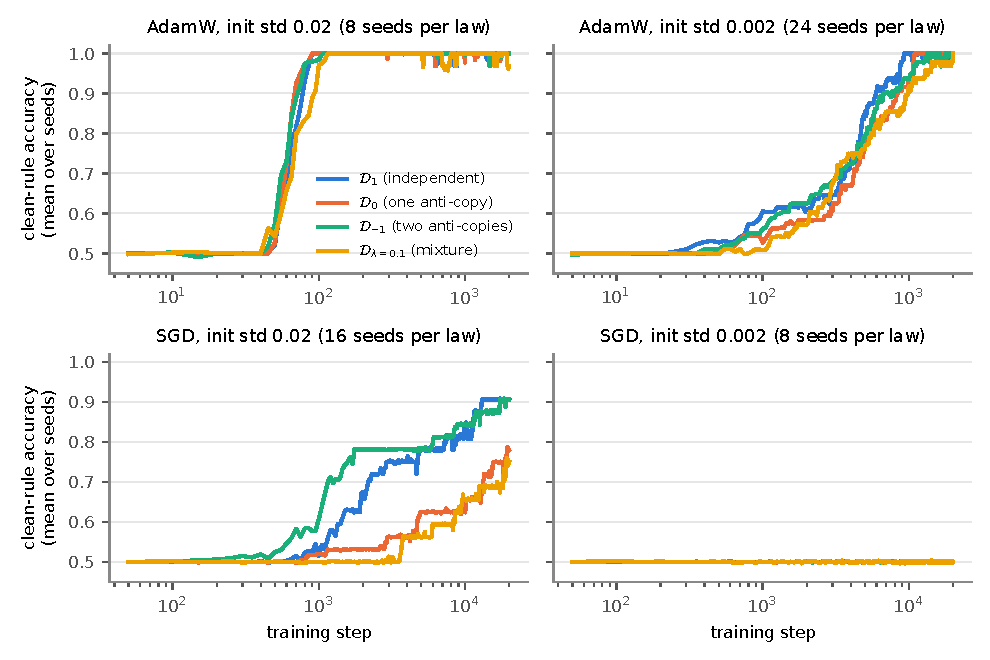
\includegraphics[width=0.9\linewidth]{figures/standard_transformer.pdf}
\caption{A standard two-layer Transformer separates the laws only under SGD. Mean clean-rule accuracy over seeds for the four laws,
AdamW and SGD at two initialization scales.}
\label{fig:standard}
\end{figure}

\section{Experimental results in detail}
\label{app:experiments}
\paragraph{Does the network produce the derived gradients?}
We first instantiate the matrices and residual paths of \cref{sec:architecture}, rather than directly coding its reduced logit.
Across 72 configurations spanning three context sizes, four cancellation coefficients, two losses, and three score/weight settings,
autograd agrees with the analytical logits and velocities to absolute tolerance $10^{-12}$.
This checks both the neural realization and the factor of two arising from the two trainable score groups.
All supported prefixes and errors are enumerated with their exact masses, so there is no sampling variability (\cref{app:network-experiments}).
The flow itself can also be run through the network: we integrate the four tied coordinates $(q_s,q_d,r_1,r_2)$ along
$-\nabla\mathcal L$ computed by automatic differentiation through the explicit matrices, by DOP853 (relative tolerance $10^{-10}$), from \cref{eq:initialization} until
source attention reaches $\tfrac12$. For $N=16$, $\kappa\in\{1,0\}$, $\varepsilon\in\{0.03,0.01,0.003\}$ and both losses, the $12$ routing times agree with the reduced
flow to relative error at most $1.9\times10^{-9}$, and $r_1-r_2$ and $q_s+q_d$ stay below $5\times10^{-14}$, so the reduced trajectories are those of the network.
The same check runs the causal model of \cref{thm:causal}: correlation loss averaged over the $N$ supervised prefixes, the flow stopped when every prefix routes.
For $N\in\{8,16\}$, the clean, independent and cancelling regimes ($\eta=0.2$ for the noisy ones) and $\varepsilon\in\{0.03,0.01\}$, the $12$ routing times agree with the reduced
causal flow to relative error at most $2\times10^{-11}$.

\paragraph{Matched loss comparison.}
\Cref{tab:network-flow} reports continuous gradient-flow times at error probability $0.1$.
The initialization, context size, population law, stopping rule and parameter metric are held fixed between the two losses.
The correlation runs test \cref{thm:separation}(i)--(ii); the cross-entropy runs test the escape orders of \cref{thm:separation}(iv)
and the complete routing that we verify only numerically.
\Cref{fig:network-flow} separately displays escape to score gap $0.01$ and routing to source attention $\tfrac{1}{2}$.

\begin{table}[t]
\centering\small
\caption{Matched population-flow experiment in the derived one-block parameterization.
Error probability $\eta=0.1$. Subscripts $1$ and $0$ denote the independent law $\Dlaw1$ and the anti-copy law $\Dlaw0$.
All columns are continuous gradient-flow time.}
\label{tab:network-flow}
\fitwidth{\begin{tabular}{@{}rr rrrr@{}}
\toprule
$N$ & $\varepsilon$ & $T_{\mathrm{corr},1}$ & $T_{\mathrm{corr},0}$ & $T_{\mathrm{ce},1}$ & $T_{\mathrm{ce},0}$\\
\midrule
16 & 0.03 & 133.1 & 1,380.0 & 140.9 & 1,406.8\\
16 & 0.01 & 176.9 & 4,316.4 & 184.8 & 4,351.2\\
16 & 0.003 & 225.0 & 14,655.1 & 232.9 & 14,698.7\\
16 & 0.001 & 269.0 & 44,248.7 & 276.9 & 44,300.3\\
64 & 0.03 & 520.6 & 5,480.0 & 546.4 & 5,593.7\\
64 & 0.01 & 695.9 & 17,214.8 & 721.7 & 17,363.5\\
64 & 0.003 & 888.5 & 58,557.6 & 914.3 & 58,745.0\\
64 & 0.001 & 1,064.3 & 176,921.0 & 1,090.1 & 177,143.8\\
\bottomrule
\end{tabular}
}
\end{table}
\begin{figure}[t]
\centering
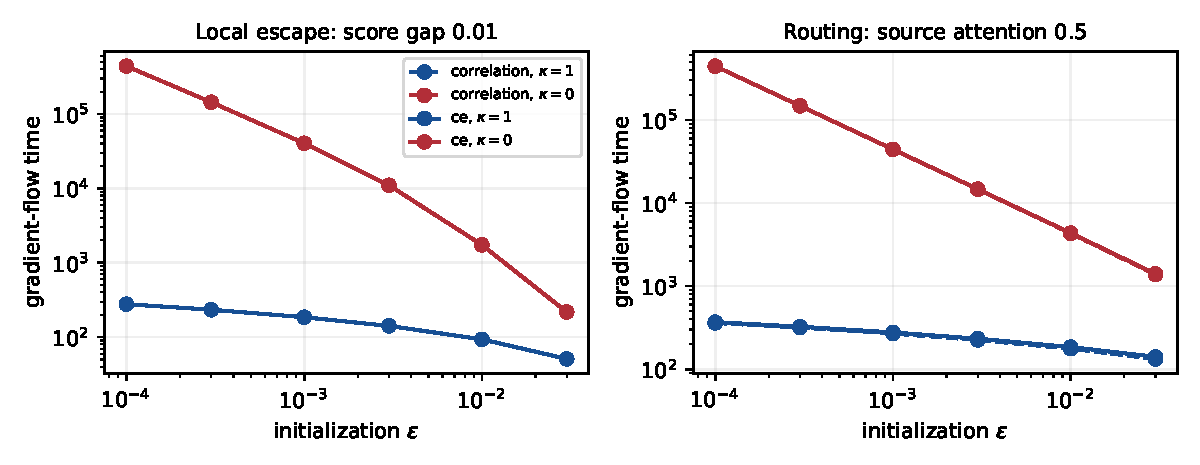
\includegraphics[width=\linewidth]{figures/one_block_scaling.pdf}
\caption{Separate tests of escape and full routing. Context size $N=16$, error probability $\eta=0.1$.
Dashed curves use correlation loss and solid curves use cross-entropy, with otherwise matched settings.
The theorem predicts distinct initialization orders for both local escape and complete routing.}
\label{fig:network-flow}
\end{figure}

\paragraph{The exact quadrature.} Direct integration of the flow of \cref{lem:invariant} agrees with \cref{eq:time} to five significant
figures, and the conserved quantity drifts by at most $6\times10^{-9}$, for $N\in\{16,64,256\}$ and $\varepsilon\in\{10^{-2},10^{-3}\}$;
every bound of \cref{thm:separation} holds (\cref{tab:quadrature}). Over-cancellation follows the exact criterion of
\cref{thm:separation}(iii): at $N=64$ and $\varepsilon=0.01$, routing completes at $\kappa=-0.007$, where $-F(q_0)<\varepsilon^2$, and does not
complete at $\kappa=-0.0283$, where $-F(q_0)\simeq3.9\times10^{-4}>\varepsilon^2$. The routing time is linear in $N$ under both laws. Reducing
$\varepsilon$ tenfold multiplies $\Tr(\Dlaw0)$ by $10.3$ and $\Tr(\Dlaw1)$ by $1.5$.

\begin{figure}[t]
\centering
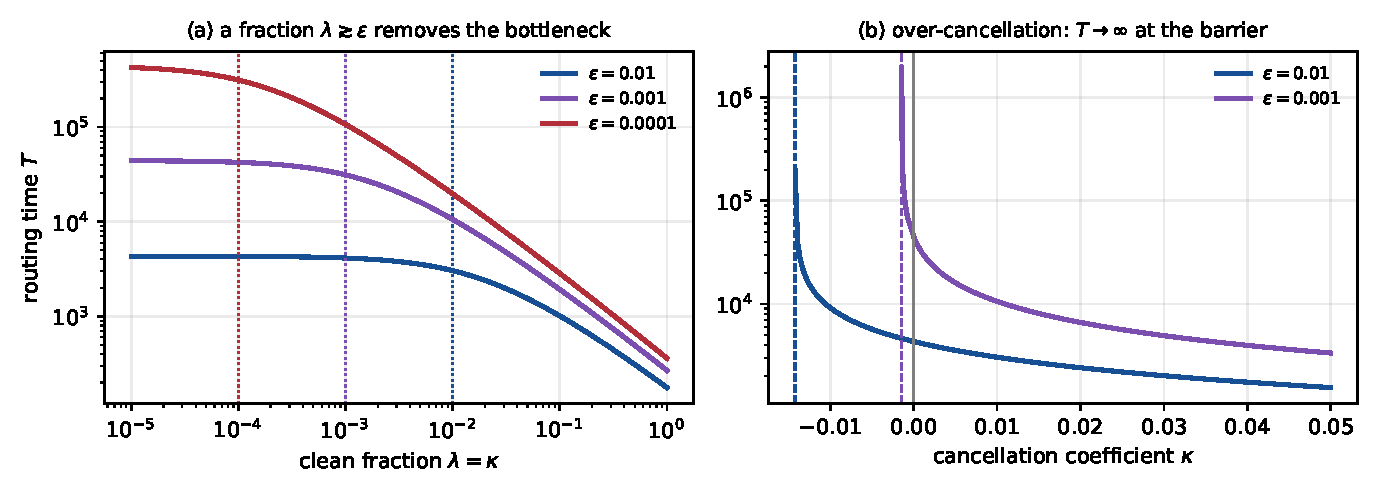
\includegraphics[width=\linewidth]{figures/kappa_sweep.pdf}
\caption{Routing time across the cancellation coefficient, correlation loss, $N=16$, $\eta=0.1$, exact quadrature.
(a) Diluting the anti-copy law with a clean fraction $\lambda=\kappa$: the plateau at $\Theta(\tfrac{1}{\varepsilon})$ ends near $\lambda\approx\varepsilon$ (dotted lines).
(b) Through $\kappa=0$ into over-cancellation: the routing time diverges at the barrier $\varepsilon^2=-F(q_0)$ (dashed lines), at $\kappa\approx-1.4\,\varepsilon$.}
\label{fig:kappa}
\end{figure}

\paragraph{Diluting the cancellation.} We integrate the primitive and the routing time together for $\kappa\in[-1,1]$ (\cref{fig:kappa}).
For clean fractions $\lambda\in[0,1]$, $N\in\{16,64\}$ and $\varepsilon\in\{10^{-2},10^{-3},10^{-4}\}$, the exact routing time stays within a factor $1.03$--$1.51$ of
$\tfrac{N-1}{\gamma}\int_0^1\tfrac{dq}{\varepsilon^2+\lambda q+q^2}$, the quantity that \cref{cor:dilution} evaluates. At $N=16$ the over-cancellation barrier sits at
$\kappa=-0.0142$ for $\varepsilon=10^{-2}$ and at $\kappa=-0.00141$ for $\varepsilon=10^{-3}$.

\begin{table}[t]
\caption{Exact routing times of the correlation-loss flow. $\gamma=1$. ODE: direct integration; quadrature: \cref{eq:time}; drift:
largest deviation of $r^2-F(q)-\varepsilon^2$ along the trajectory.}
\label{tab:quadrature}
\centering\small
\begin{tabular}{@{}rr rr rr r@{}}
\toprule
 & & \multicolumn{2}{c}{$\Dlaw1$} & \multicolumn{2}{c}{$\Dlaw0$} & \\
\cmidrule(lr){3-4}\cmidrule(lr){5-6}
$N$ & $\varepsilon$ & ODE & quadrature & ODE & quadrature & ratio\\
\midrule
16  & $10^{-2}$ & 141.5  & 141.5  & 3{,}453   & 3{,}453   & 24\\
16  & $10^{-3}$ & 215.2  & 215.2  & 35{,}399  & 35{,}399  & 164\\
64  & $10^{-2}$ & 556.8  & 556.8  & 13{,}772  & 13{,}772  & 25\\
64  & $10^{-3}$ & 851.4  & 851.4  & 141{,}540 & 141{,}540 & 166\\
256 & $10^{-2}$ & 2{,}215 & 2{,}215 & 55{,}043  & 55{,}043  & 25\\
256 & $10^{-3}$ & 3{,}394 & 3{,}394 & 566{,}080 & 566{,}080 & 167\\
\bottomrule
\end{tabular}
\end{table}

\paragraph{Does the causal error process match the new theorem?}
The causal check propagates the exact finite-state law of the prefix sum and final sign.
For $\eta=0.2$ and $N\in\{8,16,32\}$, it checks every supervised position's local error rate, cancellation coefficient, and the cancelling variance recurrence.
Propagating the error count jointly with these states also verifies the binomial law and the high-probability bound.
An additional 18 matrix-gradient configurations enumerate both instructions and both error signs under the history-dependent kernel.
The largest gradient discrepancy is below $10^{-12}$; there is no Monte Carlo estimation.
\Cref{tab:causal-flow} reports 36 averaged-loss routing runs across fully correct, independently corrupted and structured corrupted supervision.
All three share the initialization, seed and instruction process; the two noisy regimes share $\eta=0.2$.
Nine further matrix configurations verify the fully correct control.
The independent-noise times agree with $T_{\mathrm{clean}}/(1-2\eta)$ to relative error below $10^{-10}$.
The expected incorrect fraction is $0.1125$, $0.10625$, and $0.103125$ for $N=8,16,32$, respectively, approaching $0.1$.
For $N=16$, reducing $\varepsilon$ from $0.01$ to $0.001$ increases routing time by a factor $1.52$ with independent errors and $10.26$ with cancelling errors.
All runs satisfy the explicit bounds in \cref{app:trace-proof}.
At $N=16$ and $\varepsilon=0.01$, eight additional runs sweep $\eta\in\{0.1,0.2,0.3,0.4\}$ in the two noisy regimes.
The rescaled times $(1-2\eta)T$ remain constant to relative error below $10^{-10}$: about $207.9$ for independent errors and $5{,}089.6$ for structured errors.

\begin{table}[t]
\centering\small
\caption{Correct computation from clean and corrupted reasoning supervision. The clean control has no errors; both noisy regimes have local error rate $\eta=0.2$.
The same block parameters train on all $N$ selected positions. Times reach source attention $\tfrac{1}{2}$ on every prefix; the final column compares structured errors with clean supervision.}
\label{tab:causal-flow}
\begin{tabular}{@{}rr rrrr@{}}
\toprule
$N$ & $\varepsilon$ & clean & independent & structured & ratio to clean\\
\midrule
8 & 0.03 & 81.3 & 135.6 & 1,393.2 & 17.1\\
8 & 0.01 & 107.8 & 179.7 & 4,347.9 & 40.3\\
8 & 0.003 & 136.8 & 228.1 & 14,747.2 & 107.8\\
8 & 0.001 & 163.4 & 272.3 & 44,511.6 & 272.5\\
16 & 0.03 & 156.1 & 260.2 & 2,708.0 & 17.3\\
16 & 0.01 & 207.9 & 346.5 & 8,482.6 & 40.8\\
16 & 0.003 & 264.7 & 441.2 & 28,819.0 & 108.9\\
16 & 0.001 & 316.6 & 527.6 & 87,034.8 & 274.9\\
32 & 0.03 & 305.2 & 508.7 & 5,336.7 & 17.5\\
32 & 0.01 & 407.5 & 679.2 & 16,752.4 & 41.1\\
32 & 0.003 & 519.9 & 866.5 & 56,967.0 & 109.6\\
32 & 0.001 & 622.5 & 1,037.5 & 172,097.6 & 276.5\\
\bottomrule
\end{tabular}

\end{table}

\paragraph{Does the separation survive untying?}
We next train every entry of the one-block network independently: all seven-by-seven query, key, value and output matrices,
both MLP layers with their bias, and the readout, under binary cross-entropy on the exact population of $\Dlaw\kappa$, $N=16$, $\eta=0.1$.
Three initialization families move progressively away from the theorem.
(A) The directions of \cref{sec:architecture} with random magnitudes: fixed directions get magnitudes in $[\tfrac{1}{2},2]$,
each of the eight MLP rule entries gets $\varepsilon$ times a magnitude in $[\tfrac{1}{2},2]$, with a random sign per layer, and the four MLP units are no longer tied.
(B) The same plus independent Gaussian noise of fan-in scale $0.1$ or $0.3$ on every matrix.
(C) Fan-in Gaussian matrices scaled by $\varepsilon$, a sixteen-unit MLP, and nothing hand-coded.
Full-batch gradient descent with backtracking measures time on the gradient-flow clock (\cref{app:network-experiments}).

\Cref{tab:untied} reports how many of three seeds reach $99\%$ clean-rule accuracy within flow time $3\times10^4$.
With clean supervision, every seed of family (B) learns at every $\varepsilon\le0.1$, within $51$ time units,
and two of three seeds of family (A) learn at every $\varepsilon\le0.5$; the third starts with opposite rule-factor signs in the two MLP layers and fails at every $\varepsilon$.
Exact cancellation stalls: with noise, no seed learns below $\varepsilon=0.1$ ($0.1$ noise) or $\varepsilon=0.5$ ($0.3$ noise);
without noise, the seeds that learn slow down roughly as $\tfrac{1}{\varepsilon}$, from $24$ time units at $\varepsilon=0.3$ to $2{,}514$ at $\varepsilon=0.003$.
Over-cancellation fails at every $\varepsilon\le0.3$ and recovers only at $\varepsilon\ge0.5$ ($\varepsilon=1$ with $0.3$ noise),
the untied counterpart of the barrier in \cref{thm:separation}(iii).
In family (C), with three seeds and gradient descent, the three laws do not separate clearly; the next paragraph tests this regime at scale.

\paragraph{Does the full-matrix plateau appear?}
We train every entry from exactly $W_0$, $N=16$, $\eta=0.1$, by gradient descent with step $0.5$, and records the first flow time at which
$\|W-W_0\|_F=\varepsilon$. Under the anti-copy law the exit time is $1{,}048$, $1{,}579$, $3{,}170$, $6{,}351$, $10{,}592$ and $15{,}893$ for
$\varepsilon=0.03,0.02,0.01,0.005,0.003,0.002$, that is between $31.4/\varepsilon$ and $31.8/\varepsilon$, and the largest $|\E[yz_W]|$ inside the ball is $0.065\,\varepsilon^3$ at every $\varepsilon$:
the order of \cref{thm:fullmatrix}, with a much smaller constant than the proved $\gamma C_B=528$. Under the independent law every run leaves the ball at flow time $23$,
whatever $\varepsilon$ is, and its correlation inside the ball scales as $\varepsilon^2$. The full-matrix network can therefore escape quickly when credit is not cancelled.
A variant pads the embeddings and $W_0$ with zeros to residual width $D$ and trains every $D$-dimensional matrix.
From exactly $W_0$ the padded coordinates receive zero gradient and stay zero, so widths $16$ and $64$ reproduce the numbers above exactly.
A second variant starts instead from $W_0$ plus a Gaussian perturbation of Frobenius norm $\varepsilon^{3/2}$ spread over every entry, padded ones included,
the setting of \cref{thm:fullmatrix}(iii). At widths $7$, $16$ and $64$, the anti-copy law then leaves the ball at flow time between $20.2/\varepsilon$ and $26.5/\varepsilon$,
the largest $|\E[yz_W]|$ inside it is at most $0.105\,\varepsilon^3$, and the independent law still leaves at flow time $22.5$--$23$ for every $\varepsilon$.

\paragraph{From fully random initialization.}
We repeat family (C) with ten seeds, $N\in\{8,16,32\}$, $\varepsilon\in\{0.05,0.1,0.2,0.3,0.5,0.7,1,1.5\}$, and two optimizers: backtracking gradient descent with
flow-time budget $10^5$, and Adam with step size $3\times10^{-3}$ for $10^5$ steps (\cref{tab:randinit}).
The first escape from chance takes the same time under every law (for Adam, a median of $45$, $52$ and $60$ steps at $N=8,16,32$, within a few steps across $\kappa$):
from random matrices it is limited by the product of small weights, not by the data, as in deep linear networks.
The laws differ in where training goes next. With Adam, all $240$ runs on the independent law reach the Bayes predictor; on the anti-copy law $33$--$40\%$ of runs
stall, and with two anti-copies $43$--$50\%$. All $195$ stalled runs are flat, with loss changing by less than $10^{-4}$ over the last $4\times10^4$ steps, and $193$ of them sit at a single stationary point
for each law and context size, with loss $0.43$--$0.50$ against the Bayes value $0.325$ and clean accuracy $79$--$91\%$. Gradient descent shows the same ordering among initializations $\varepsilon\ge0.5$, where the
independent law learns reliably. From random initialization, then, cancellation does not delay the first escape; it makes training land in a worse stationary point.
At every stalled point the mean source attention is $\tfrac12$. The point routes by instruction: when one sign of $b$ is shown, attention is on the source and the
loss is $H(\eta)$, with $H$ the binary entropy in nats; when the other is shown, the source receives no weight and the readout is the Bayes predictor of $y$ from the decoys alone. The clean accuracy is then
$\tfrac12(1+a_{\mathrm{dec}})$ and the loss $\tfrac12(H(\eta)+H(y\mid\text{decoys}))$, where $a_{\mathrm{dec}}$ is the best decoy-only accuracy. For one anti-copy these give $82.8$, $80.2$ and
$78.6\%$ with losses $0.485$, $0.498$ and $0.504$ at $N=8,16,32$; for two anti-copies, $90.6$, $85.5$ and $82.2\%$ with $0.426$, $0.468$ and $0.489$. Every
value equals the measured one to three decimals. Under the independent law the decoys carry no information about the source, so this split point gives no decoy-side
gain, consistent with no independent-law run stalling.

\paragraph{Removing the product of small weights.} Family (C$'$) keeps every matrix random but draws the query, value and output matrices at order one,
$\mathrm N(0,\tfrac{1}{\text{fan-in}})$, and only the key and both MLP layers at $\varepsilon Z/\sqrt{\text{fan-in}}$, so attention starts uniform up to $O(\varepsilon)$;
the MLP bias is either the gate value $-B$ or uniform on $\pm\tfrac{1}{\sqrt7}$, and the readout has scale $1$ or $\varepsilon$
(same $N$, $\varepsilon$, seeds and optimizers as \cref{tab:randinit}). The plateau exit again takes the same time under
every law, and it does not grow as $\varepsilon$ shrinks (at $N=16$ with gradient descent, flow time $28$--$36$ at $\varepsilon=0.05$ for all three laws), so this rescaling does not
recover the $\tfrac{1}{\varepsilon}$ delay of \cref{thm:separation}. With the random bias the laws again differ in how often training reaches $99\%$ clean-rule accuracy:
with Adam, $79$--$80$ of $80$ runs per cell under the independent law, $27$--$43$ under one anti-copy and $19$--$28$ under two. With the gate bias all three laws learn
in only $21$--$39$ of $80$.

\begin{table}[t]
\centering\small
\caption{Fully random initialization, every matrix entry trained. Anti-copy law, $\eta=0.1$, binary cross-entropy, ten seeds per initialization.
Each cell: runs reaching $99\%$ clean-rule accuracy within the budget; Adam pools eight initializations, gradient descent the four with $\varepsilon\ge0.5$.}
\label{tab:randinit}
\begin{tabular}{@{}lcccccc@{}}
\toprule
 & \multicolumn{3}{c}{Adam, all $\varepsilon$} & \multicolumn{3}{c}{GD, $\varepsilon\ge0.5$}\\
\cmidrule(lr){2-4}\cmidrule(lr){5-7}
$N$ & $\kappa=1$ & $\kappa=0$ & $\kappa=-1$ & $\kappa=1$ & $\kappa=0$ & $\kappa=-1$\\
\midrule
8 & 80/80 & 54/80 & 45/80 & 37/40 & 24/40 & 20/40\\
16 & 80/80 & 52/80 & 46/80 & 34/40 & 23/40 & 19/40\\
32 & 80/80 & 48/80 & 40/80 & 33/40 & 23/40 & 19/40\\
\bottomrule
\end{tabular}

\end{table}

\begin{table}[t]
\centering\small
\caption{Untied one-block training under the anti-copy law. Every matrix entry trains; binary cross-entropy, $N=16$, $\eta=0.1$.
Each cell: seeds (of three) reaching $99\%$ clean-rule accuracy within gradient-flow time $3\times10^4$, and their median time.
$\kappa=1$: independent decoys; $\kappa=0$: one anti-copy; $\kappa=-1$: two anti-copies.}
\label{tab:untied}
\fitwidth{\begin{tabular}{@{}llcccccc@{}}
\toprule
Initialization & $\kappa$ & $\varepsilon=0.003$ & $\varepsilon=0.03$ & $\varepsilon=0.1$ & $\varepsilon=0.3$ & $\varepsilon=0.5$ & $\varepsilon=1$\\
\midrule
A: directions & $+1$ & 2/3 (85) & 2/3 (59) & 2/3 (34) & 2/3 (14) & 2/3 (9) & 1/3 (4)\\
 & $+0$ & 1/3 (2,514) & 2/3 (497) & 2/3 (114) & 2/3 (24) & 1/3 (9) & 1/3 (4)\\
 & $-1$ & 0/3 & 0/3 & 0/3 & 0/3 & 1/3 (26) & 1/3 (4)\\
\addlinespace
B: $+\,0.1$ noise & $+1$ & 3/3 (51) & 3/3 (44) & 3/3 (34) & 2/3 (14) & 2/3 (8) & 2/3 (57)\\
 & $+0$ & 0/3 & 0/3 & 1/3 (97) & 1/3 (20) & 1/3 (10) & 1/3 (4)\\
 & $-1$ & 0/3 & 0/3 & 0/3 & 0/3 & 2/3 (454) & 1/3 (5)\\
\addlinespace
B: $+\,0.3$ noise & $+1$ & 3/3 (34) & 3/3 (34) & 3/3 (30) & 3/3 (20) & 3/3 (11) & 2/3 (19)\\
 & $+0$ & 0/3 & 0/3 & 0/3 & 0/3 & 1/3 (20) & 1/3 (6)\\
 & $-1$ & 0/3 & 0/3 & 0/3 & 0/3 & 0/3 & 1/3 (11)\\
\addlinespace
C: random & $+1$ & 0/3 & 0/3 & 1/3 (26,330) & 1/3 (1,009) & 2/3 (168) & 3/3 (44)\\
 & $+0$ & 0/3 & 0/3 & 1/3 (23,109) & 1/3 (885) & 1/3 (211) & 2/3 (21)\\
 & $-1$ & 0/3 & 0/3 & 1/3 (23,109) & 1/3 (885) & 1/3 (185) & 2/3 (22)\\
\bottomrule
\end{tabular}
}
\end{table}


\end{document}
